% Copyright (c)  2005-2009  EDF-EADS-PHIMECA.
% Permission is granted to copy, distribute and/or modify this document
% under the terms of the GNU Free Documentation License, Version 1.2
% or any later version published by the Free Software Foundation;
% with no Invariant Sections, no Front-Cover Texts, and no Back-Cover
% Texts.  A copy of the license is included in the section entitled "GNU
% Free Documentation License".

\documentclass[a4paper,11pt]{article}

\usepackage{latex2html}
\usepackage[T1]{fontenc}
\usepackage[latin1]{inputenc}
\usepackage{graphicx,color,listings}
\usepackage{fancyhdr}
\usepackage{amsmath, amssymb}
% \DeclareGraphicsExtensions{.png}
\usepackage{ifpdf}

\setlength{\textwidth}{18.5cm}
\setlength{\textheight}{23cm}
\setlength{\hoffset}{-1.04cm}
\setlength{\voffset}{-1.54cm}
\setlength{\oddsidemargin}{0cm}
\setlength{\evensidemargin}{0cm}
\setlength{\topmargin}{0cm}
\setlength{\headheight}{1cm}
\setlength{\headsep}{0.5cm}
\setlength{\marginparsep}{0cm}
\setlength{\marginparwidth}{0cm}
\setlength{\footskip}{1cm}
\setlength{\parindent}{0cm}

\pagestyle{fancy}
\fancyhf{} \rhead{\bfseries \thepage} \lhead{\bfseries \nouppercase Wrappers Guide}
\rfoot{\bfseries \copyright 2005-2012 EDF - EADS - PhiMeca} \lfoot{}

% package url is used in the bibliography for URL layout
\usepackage{url}

% fonts for the table and figure captions
% \usepackage[small,bf,up]{caption}
% \renewcommand{\captionfont}{\small\itshape}

% depth of the TOC
\setcounter{tocdepth}{4}

% macros used in the document
\newcommand{\OT} {Open TURNS}
\def\R{\mathbb{R}}

% index
\usepackage{makeidx}
\makeindex

\begin{document}

\begin{titlepage}
  \vspace*{2cm}
  \begin{center}
    {\huge \bf Open TURNS -- Wrappers Guide}
    \input{GenericInformation.tex}
  \end{center}
\end{titlepage}

\newpage
% Copyright (c)  2005-2009  EDF-EADS-PHIMECA.
% Permission is granted to copy, distribute and/or modify this document
% under the terms of the GNU Free Documentation License, Version 1.2
% or any later version published by the Free Software Foundation;
% with no Invariant Sections, no Front-Cover Texts, and no Back-Cover
% Texts.  A copy of the license is included in the section entitled "GNU
% Free Documentation License".
\vspace{0.5in}
\begin{center}
  \fontshape{sc} \large \centering
  \OT\ project: Coupling mechanisms with computational codes \\
  \vspace{0.3in}
  \emph{\fontshape{sc} Abstract}
  \vspace{0.5in}
\end{center}

The purpose of this document is to present the latest features developed within the \OT\ library regarding the interfacing mechanism with a computational code.

The latest advances offer users:
\begin{itemize}
\item greater simplicity of implementation with the use of macros and shared functions that cover a large part of the expressed needs;
\item greater reliability, again thanks to these shared functions;
\item faster development by reducing the amount of programming required from the user;
\item simplified maintenance, again thanks to the reduction of the volume of code;
\item improved performance by using parallel techniques in a few relevant spots.
\end{itemize}


\cleardoublepage
\tableofcontents
\cleardoublepage


\cleardoublepage

\section{Introduction}
% Copyright (c)  2005-2009  EDF-EADS-PHIMECA.
% Permission is granted to copy, distribute and/or modify this document
% under the terms of the GNU Free Documentation License, Version 1.2
% or any later version published by the Free Software Foundation;
% with no Invariant Sections, no Front-Cover Texts, and no Back-Cover
% Texts.  A copy of the license is included in the section entitled "GNU
% Free Documentation License".

\emph{We would like to thank Vincent Lefebvre and Olivier Morvant from the Descartes project, who are the original authors of this document that we have almost entirely drawn upon.}

\subsection{Document goals}
The coding rules edicted in this document mainly regard:
\begin{itemize}
\item the structure of modules and classes;
\item the names of the source files;
\item the use of the C++ and Python programming languages;
\item the documentation included inside the source files;
\item the format used to write statements in the programming languages.
\end{itemize}

The purpose of these rules is to provide a common formalism for the project in order to help the developers produce code that is globally homogeneous, readable, understandable by all and also efficient and reliable, respecting the architectural choices and constraints established to produce the code of the \OT\ project. The scope of this document only embraces files produced in the \OT\ project and does not apply to external software included in the project \emph{as is}.

\subsection{Conventions}
This paragraph establishes the conventions used in this document.

Each coding rules is identified by a unique number prefixed by the letter R.
\RuleX{xx}{<Description of rule>}
Examples of source code in C++ and Python are framed. Correct examples are given in blue, while incorrect examples are in red.

\lstset{language=C++, basicstyle=\normalsize}
\begin{lstlisting}[frame=TRL]
  <Example>
  ...
\end{lstlisting}
\lstset{language=C++, basicstyle=\color{blue}}
\begin{lstlisting}[frame=RL]
  <correct example>
  ...
\end{lstlisting}

\lstset{language=C++, basicstyle=\color{red}}
\begin{lstlisting}[frame=RLB]
  <incorrect example>
  ...
\end{lstlisting}

When an example requires comments, these are given above the said example and they appear in italics.

\emph{Comment about example}
\lstset{language=C++, basicstyle=\normalsize}
\begin{lstlisting}[frame=TRBL]
  <Example>
\end{lstlisting}

Elements from the text, rules or source code cited as an example and appearing between the two characters {\bf <} and {\bf >} correspond to a description of the expected items or objects. The following example shows that {\bf <condition>} represents a boolean expression and the function {\bf compute} is called on a piece of data of type length, with its default unit.

\begin{lstlisting}[frame=TRBL]
  if ( <condition> ) {
    r = compute( <length in cm> )
  }
\end{lstlisting}

By extension, the following symbols are used to describe a grammar, a call syntax, etc.

\begin{tabular}{rl}
  {\bf <real>} & a real number \\
  {\bf <integer>} & an integer \\
  {\bf <string>} & a string \\
  {\bf <filename>} & a string representing a filename
\end{tabular}

The first rule is given below this introductory paragraph and deals with the language used in the code.
\Rule{Coding language}{{\bf Coding language:} the language used to program classes, functions and modules in \OT\ is English. The comments included in the source code shall be written in English as well.}


\cleardoublepage

\section{The different types of functions}
% Copyright (c)  2005-2009  EDF-EADS-PHIMECA.
% Permission is granted to copy, distribute and/or modify this document
% under the terms of the GNU Free Documentation License, Version 1.2
% or any later version published by the Free Software Foundation;
% with no Invariant Sections, no Front-Cover Texts, and no Back-Cover
% Texts.  A copy of the license is included in the section entitled "GNU
% Free Documentation License".

Complexity does not always come from the technical side. The spoken language is the first \index{data structure}difficulty that must be overcome in computer science. In the case we are dealing with (i.e. the use of the \OT\ platform to carry out uncertainty treatment studies), we are faced with the language's poor ability to express, through specific and distinct words, concepts that are very different from each other.

The \index{data structure}difficulty that is hardest to tackle is the use of the word \emph{\index{function}function}, on which we rely quite frequently. It covers here at least three concepts.

The first meaning that we can associate with the term \emph{\index{function}function} is mathematical. In the field of the treatment of uncertainties, we are required to manipulate a mathematical function that is most often a physical model relying on input variables and producing output variables. Also known as a (broadly defined) \emph{solver}, it is the component that performs the computation in the code with which the \OT\ platform was coupled. As a mathematical object, this is a $\R^{n} \to \R^{p}$ function, where $n$ and $p$ repectively represent the number of input and output variables. When the computational code provides the \index{gradient}gradient or the \index{hessian}hessian of this function, \OT\ is expected to be able to make good use of it. \index{gradient}Gradient and \index{hessian}hessian appear in \OT\ as other mathematical functions of types $\R^{n} \to \R^{p} \times \R^{n}$ and $\R^{n} \to \R^{p} \times \R^{n} \times \R^{n}$.

To bring together these three mathematical functions linked by derivation relations in an object that allows easy handling by the users of the platform, we introduced a second concept of \emph{\index{function}function} which is mainly related to the field of uncertainty. This function is a computer object which rounds up the three mathematical objects into a consistent whole. This object makes it possible to tell the \OT\ platform that this \index{gradient}gradient function is indeed the gradient of that mathematical function.

The third concept associated with the term \emph{\index{function}function} is programming related. It is the concept of method in object programming, or of sub-program in procedural programming. This is the place to define the treatments to be carried out.

In this document, in order to distinguish these three concepts, we will use conventions designed to remove any ambiguity.

The concept of mathematical \index{function}function is called either \index{Function}Function, or \index{Gradient}Gradient or \index{Hessian}Hessian (with a capital letter) depending on its role.

The concept of unifying \index{function}function, bringing together the previous three functions, will be called \index{NumericalMathFunction}NumericalMathFunction, NMF in short, so as to remain consistent with the naming of objects within the \OT\ platform.

The concept of programming \index{function}function will simply be called function. When we need to describe an example of such function, we will use lowercase and a bold font as follows. Example: {\bf \index{prefix}\index{central term}func\_exec\_m}.

We shall see later that these three function types are closely intertwined in the \OT\ platform.

\cleardoublepage

\section{The wrapper}
% Copyright (c)  2005-2010 EDF-EADS-PHIMECA.
% Permission is granted to copy, distribute and/or modify this document
% under the terms of the GNU Free Documentation License, Version 1.2
% or any later version published by the Free Software Foundation;
% with no Invariant Sections, no Front-Cover Texts, and no Back-Cover
% Texts.  A copy of the license is included in the section entitled "GNU
% Free Documentation License".

\subsection{Operating principle of a \index{wrapper}wrapper}

\subsubsection{Why use a \index{wrapper}wrapper?}

Among the goals that the \OT\ platform attempts to reach, genericity is central. It is at the heart of the tool as it is at the heart of mathematics, which is the source of all the implemented algorithms. Therefore, an essential part of \OT\ implies that the problem to be solved, and for which we wish to conduct an uncertainty study, can be modeled as a mathematical $\R^{n} \to \R^{p}$ \index{function}function.

This model, which we chose to call \index{Function}Function, can be implemented in various ways.

It can be directly encoded within the library that forms the base of the platform. Currently, and even if it is easily feasible, no \index{Function}Function belongs to this category. The reason is primarily practical. Which Function can be hard-coded? Why this one rather than another? Given that the tool is generic and meant to be broadly disseminated, a choice made for our needs could be a problem in another context. This is why we refused to register the Functions at the library level.

It can also be coded within an analytical formula driven by a \index{NumericalMathFunction}NumericalMathFunction. This\index{data structure} will not be detailed here. It suffices to know that the said analytical formula is not hard-coded but passed as an argument of the NumericalMathFunction, which is able to interpret and execute it. Thus, the platform can work with almost any formula given by the user.

Advancing still further towards the externalization of the computation from the library, the \index{Function}Function can be implemented in a subroutine that will be dynamically (i.e. on demand) linked to the platform during computation.

Finally, it is possible to use this subroutine not to perform the computation, but to delegate this computation to an external entity, that is to say, a computational code (see Figure 3.1).

\begin{figure}
  \begin{center}
    \ifpdf
    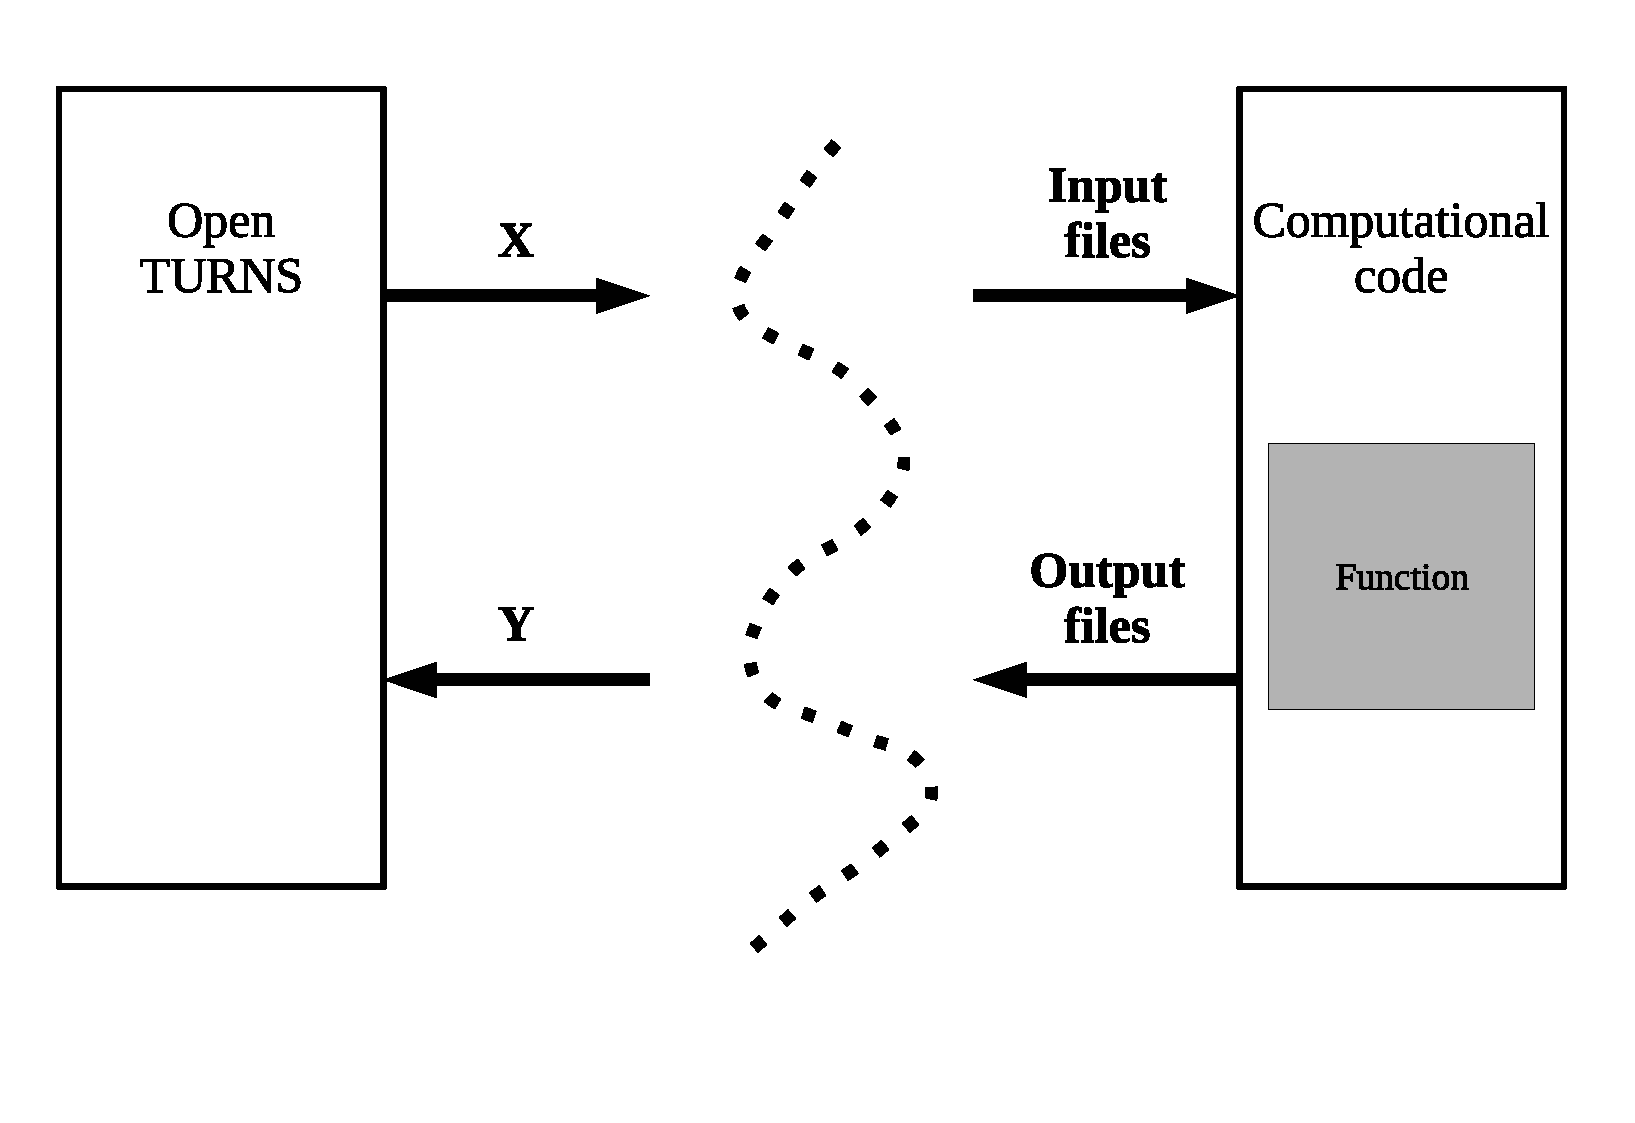
\includegraphics[width=12cm]{Figure1.pdf}
    \else
    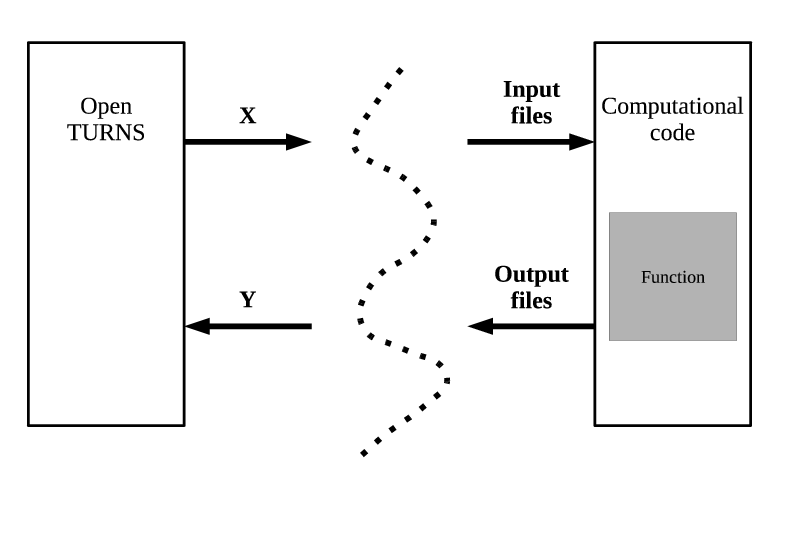
\includegraphics[width=12cm]{Figure1.png}
    \fi
    \caption[Figure 1]{Adapting the interface between \OT\ and the computational code}
  \end{center}
\end{figure}

We are therefore in a situation in which \OT\ only sees the \index{Function}Function hosted within the computational code as an object consuming a set of $n$ values (a vector \underline{X} belonging to $\R^{n}$) and producing a set of $p$ values (a vector \underline{Y} belonging to $\R^{p}$), while the computational code usually expects to receive input files and produce output files.

These files contain much more information than the $n$ or $p$ values manipulated by \OT. Moreover, they have a \index{regular expression}format that is specific to each computational code.

Therefore, it is difficult or even impossible for \OT\ adapt to all situations. It is not possible either to impose a coupling mode and force the computational codes to follow it.

If we look closer, we notice that, on the one hand, \OT\ expects the computational code to respect its interface, that is to say that it transmits the values through vectors \underline{X} and \underline{Y} and that, on the other hand, the computational code expects \OT\ to send values through its interface, that is to say its files.

The \index{wrapper}"wrapper" is precisely the subroutine that converts the interface of one element into an interface of the other, carrying out the necessary transformations on the data. In this document, we will use the word wrapper, although we could also use the more explicit but less common term "interface adapter" (see Figure 3.2).

\begin{figure}
  \begin{center}
    \ifpdf
    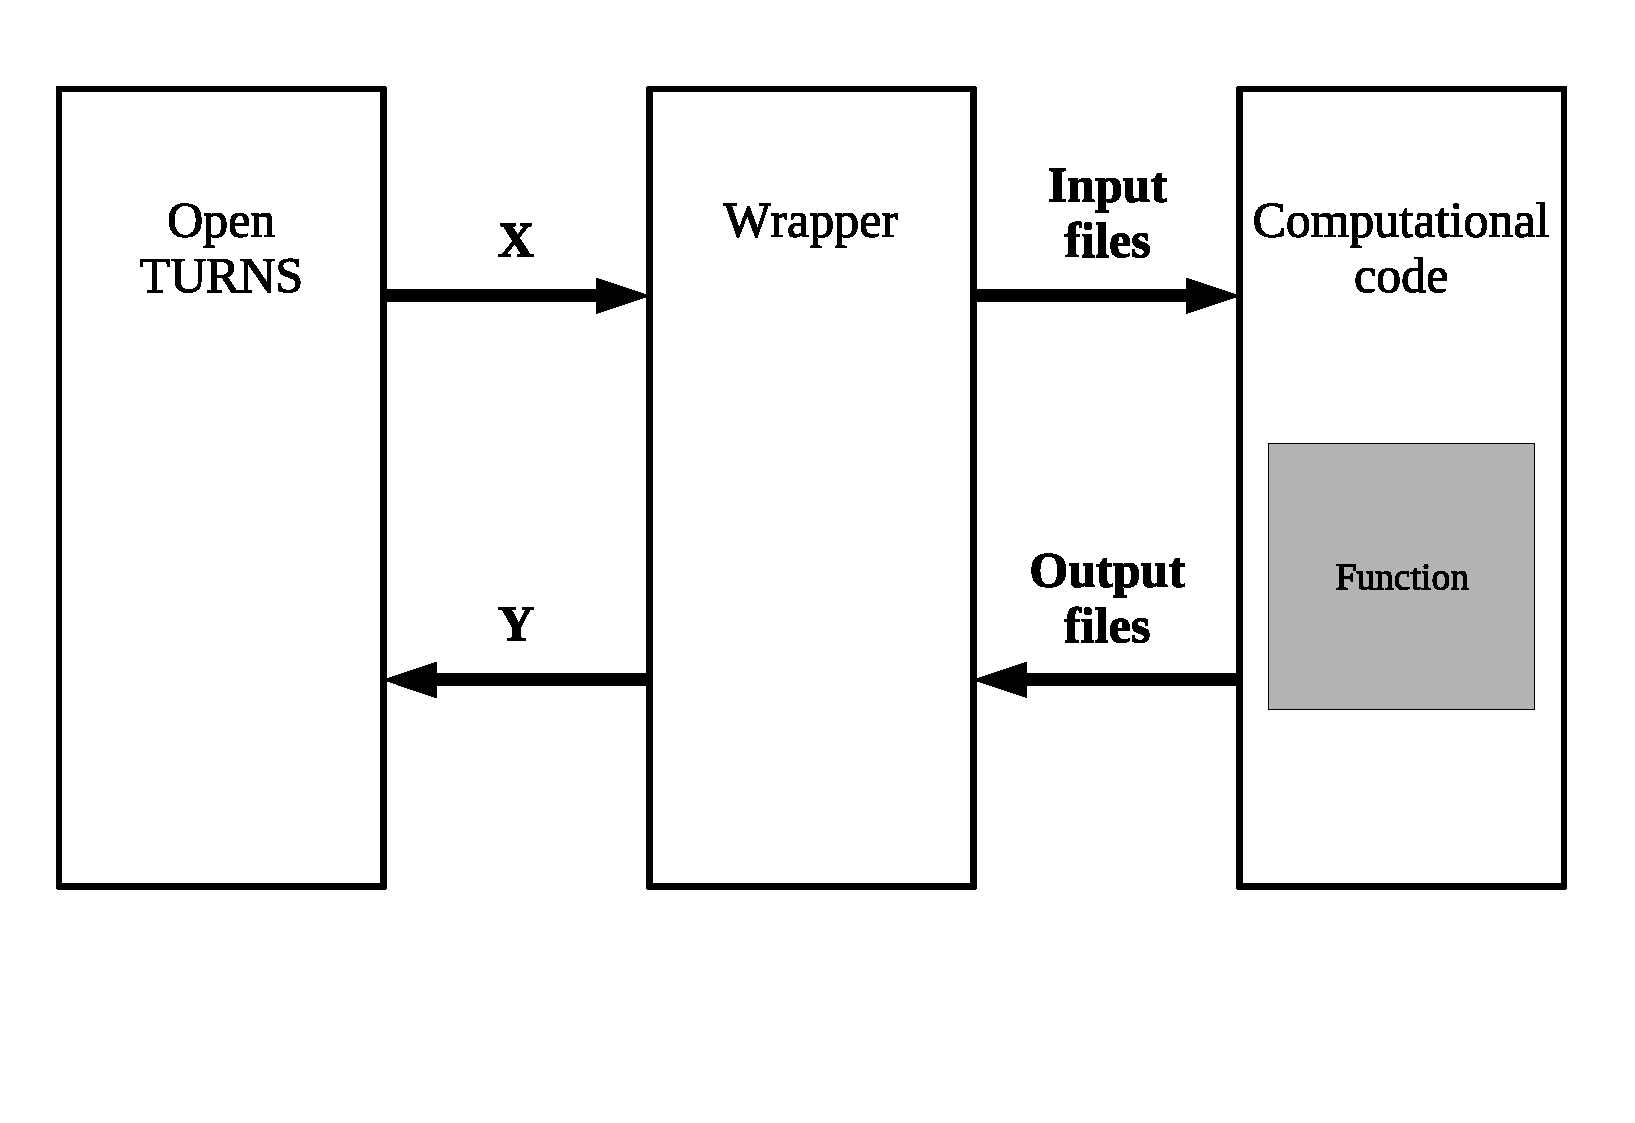
\includegraphics[width=12cm]{Figure2.pdf}
    \else
    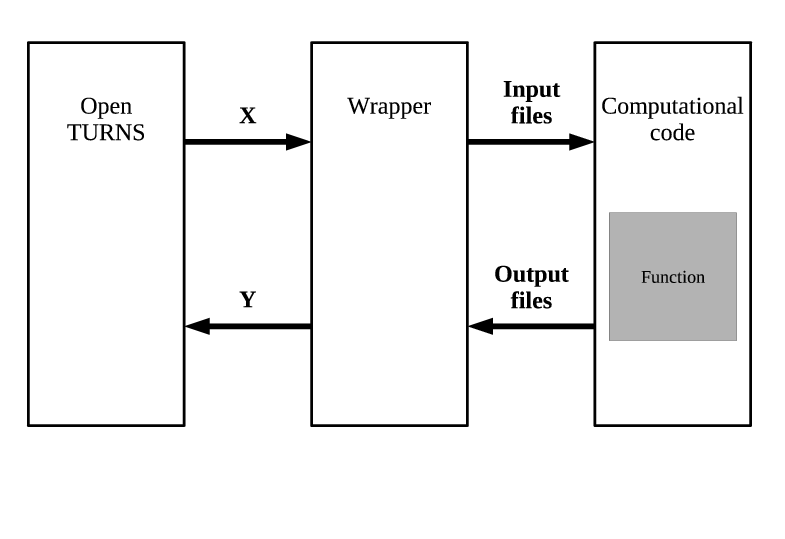
\includegraphics[width=12cm]{Figure2.png}
    \fi
    \caption[Figure 2]{Coupling a computational code using a \index{wrapper}wrapper}
  \end{center}
\end{figure}

Of the three scenarios outlined above, the \index{wrapper}wrapper is only involved in the last two. This document therefore only addresses these two cases.

As an adapter, the \index{wrapper}wrapper is not meant to change the way the user sees the computational code with which they are working. The wrapper should thus be transparent in the exchange between \OT\ and the external code. It behaves as an extension of the code towards the platform.

Beyond its role of interface adaptation, the wrapper also ensures the cooperation between a platform written in C++ and codes written in any other programming language (C, \index{FORTRAN}FORTRAN 77 or 90, Python, etc.). This\index{data structure} will be detailed later on in this document.

It is also in charge of managing the \index{execution}execution of the computational code by invoking its commands or functions at the appropriate time.

In summary, the \index{wrapper}wrapper is a variable geometry interconnection element between \OT\ and the computational code. It can be designed to provide basic or very advanced functionalities. Being specific to each code, it is its designer's responsibility to determine its capabilities.

This documentation is structured following a gradual progression. It begins by showing how to create a minimal \index{wrapper}wrapper with the most basic behavior, which will, however, be adequate in many cases; then, as the reader advances in the text, they will be able to see how to add features enriching the interface. This progression can also be regarded as a design guide for the wrapper, which will be developed in stages.

\subsubsection{Presentation of the \index{wrapper}wrapper}

Before turning to the next section, which will show how to use a \index{wrapper}wrapper, it is useful to present the elements that make it up.

From a strict computer science \index{data structure}point of view, the \index{wrapper}wrapper consists of two files:
\begin{itemize}
\item a \index{dynamic library}dynamic library compiled from a source file written in C language (eg {\bf \index{wrapper}wrapper.so})
\item a \index{description file}file describing the library in XML (eg {\bf \index{wrapper}wrapper.xml}).
\end{itemize}

Unless otherwise specified, when we speak of the \index{wrapper}wrapper in this document, we always refer to both of these files.

\subsubsection{The \index{dynamic library}dynamic library}

The \index{dynamic library}dynamic library contains the code performing all of the interfacing operations. It is loaded only when using the \index{wrapper}wrapper, which means that, when \OT\ starts, it has no ability to interface with any computational code. It acquires this ability by loading a wrapper. It is possible to simultaneously load several different wrappers in order to work with several computational codes. However, the dynamic library load mechanism prevents the coexistence of multiple instances of the same wrapper. Once loaded, a wrapper cannot be loaded a second time unless it has been unloaded first. This is why dynamic libraries are also called shared libraries, and the corresponding files have the Unix extension {\bf .so} for "shared object". This file can have any name but, in this document, we choose to call it {\bf wrapper.so} for convenience when we talk about it in generic terms.

\subsubsection{The \index{description file}description file}
The previous section indicated that the \index{wrapper}wrapper could be gradually expanded with additional features. However \OT\ can not easily infer, from the library that it loads, what these capabilities are and whether they should be used. That is why we add to the library file a \index{description file}description file written in XML which, as its name suggests, is there to inform the platform on the features offered by the wrapper library. For convenience and symmetry, we choose to name this file {\bf wrapper.xml} in this document.

\small
\begin{quote}
  \textit{Note: The choice of names is only intended to clarify our text. However, it is very inappropriate to use these names for a real \index{wrapper}wrapper intended to be distributed to users. Not only wouldn't the name be explicit, but that wrapper would likely clash with a counterpart carrying the same name but responsible for something completely different.\\
    Therefore, we recommend naming the said files using the external code to be "wrapped". For example, the developer of a wrapper for the Octave software could name these files {\bf octave.so} and {\bf octave.xml}.}
\end{quote}
\normalsize

\subsubsection{Invoking and loading a \index{wrapper}wrapper}

In order to gradually detail the way the \index{wrapper}wrapper operates, we will primarily focus on how it is used.

We adopt here the perspective of the user who seeks to carry out an uncertainty treatment study using a computational code that we will call {\bf Code\_X}. We do not concern ourselves yet with how to exchange variables with {\bf Code\_X}. This will be the subject of later sections.

All that interests us at this stage is to know that {\bf Code\_X}, seen from \OT, behaves like a $\R^{n} \to \R^{p}$ \index{Function}Function. It will therefore be used as follows\footnote{For the examples, we use the syntax of the Python text interface. The C++ syntax is very close and does not provide any additional information.}:
\index{NumericalMathFunction}
\lstset{language=Python, basicstyle=\normalsize}
\begin{lstlisting}[frame=TBRL]
  >>> f = NumericalMathFunction ( "Code_X" )
\end{lstlisting}

A \index{function}function {\bf f} interfaced with {\bf Code\_X} is created using the coupling mechanism of \OT.

Behind this very simple syntax hides a relatively complex series of operations that we will describe. We assume that the user is familiar with the object syntax of Python or C++ and with the standard classes of the \OT\ library\footnote{For details about the classes, see the \OT\ Reference Guide, available at {\bf http://www.openturns.org} or the online help of the platform.}.

The \index{NumericalMathFunction}NumericalMathFunction class allows to create programming objects mimicking the behavior of a real mathematical \index{Function}Function associated with its \index{Gradient}Gradient and its \index{Hessian}Hessian. It is thus possible to require an object of this type to evaluate itself at a given \index{data structure}point or to provide the value of its \index{gradient}gradient and its \index{hessian}hessian at this point. This mechanism simulates the derivation relations between these three concepts.

The above syntax calls the constructor of the \index{NumericalMathFunction}NumericalMathFunction class, passing a string to it as an argument, string indicating the code with which the user wants to interface. Following this call, and assuming that no error has occurred, the \index{wrapper}wrapper for {\bf Code\_X} will be loaded and the connection between the object {\bf f} and the wrapper will be established.

This operation is carried out in six steps.

\subsubsection{Step 1: Creation of a \index{NumericalMathFunction}NumericalMathFunction}

Everything starts with the creation of the \index{NumericalMathFunction}NumericalMathFunction object within the \OT\ library. Although the previous action is initiated from the Python language, it is immediately transcribed into C++ code executed within the library (see Figure 3.3).

\begin{figure}
  \begin{center}
    \ifpdf
    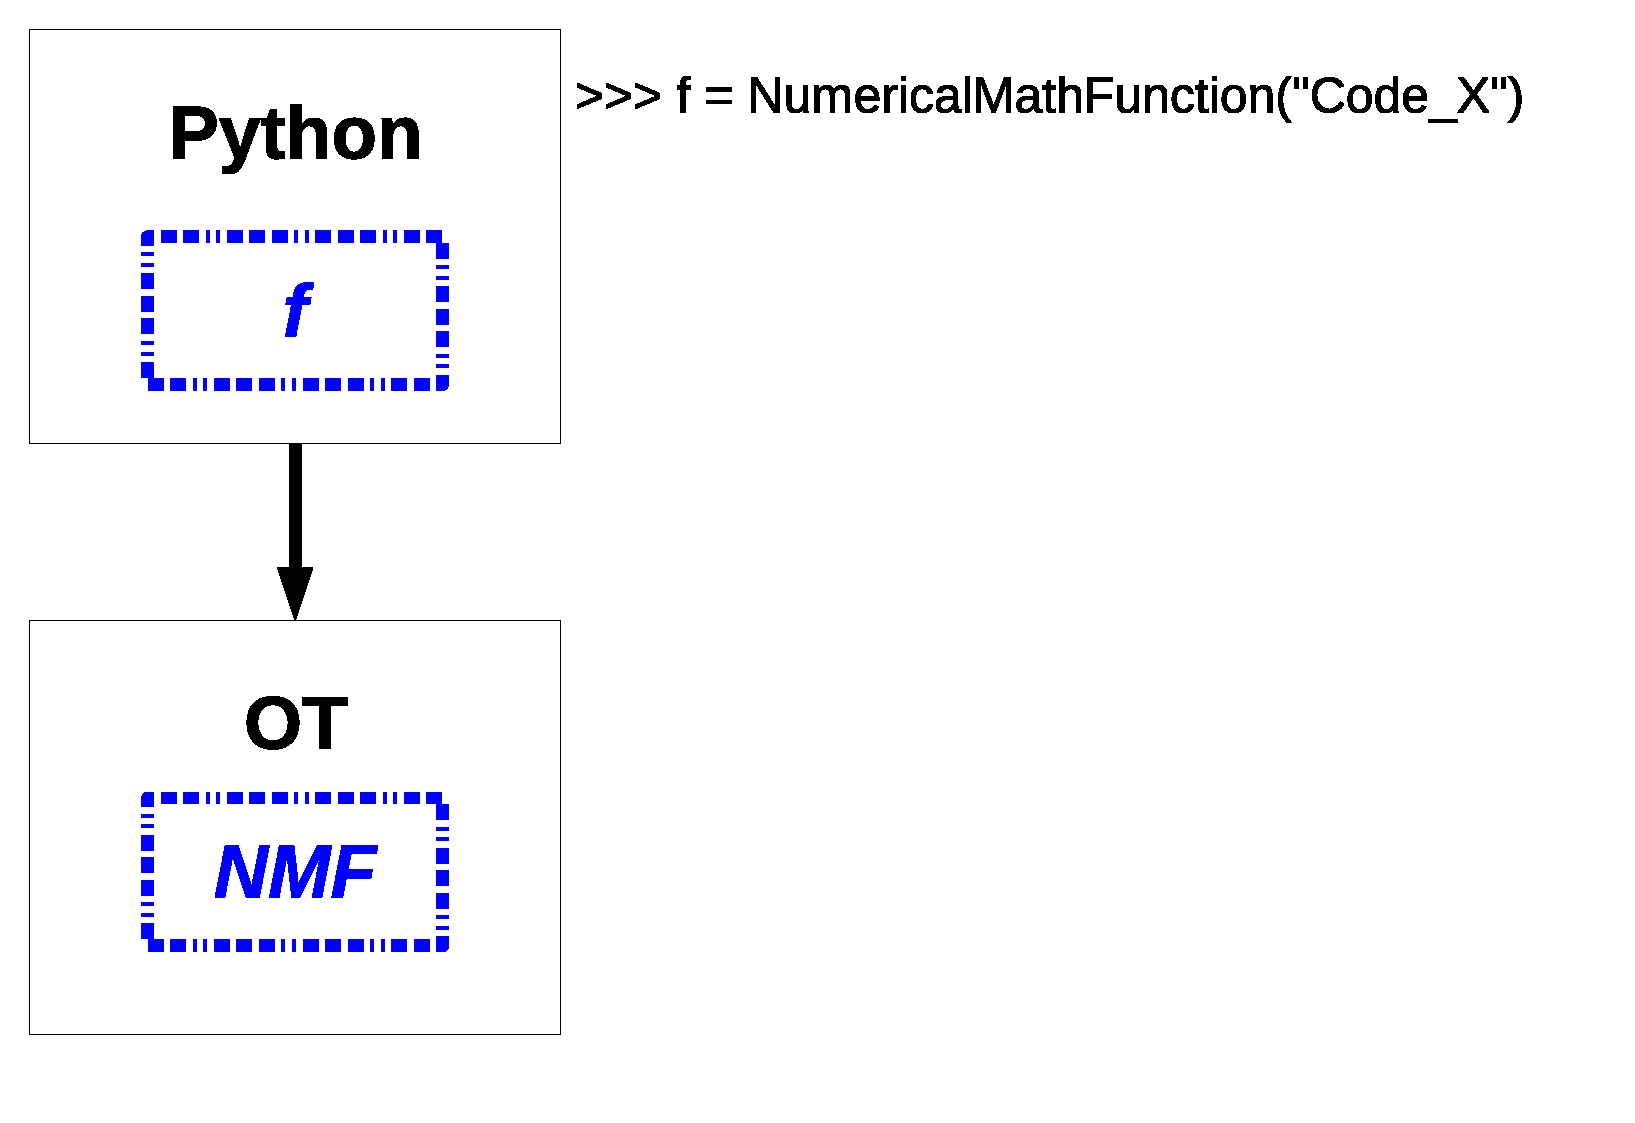
\includegraphics[width=12cm]{Figure3.pdf}
    \else
    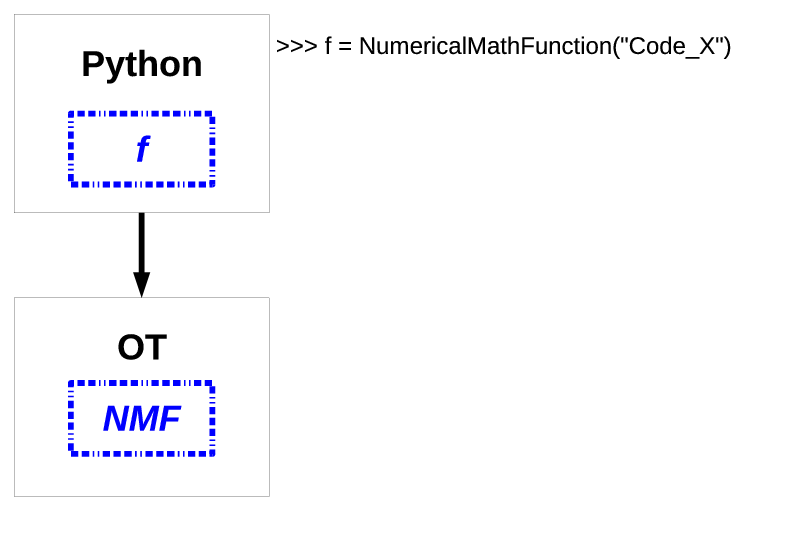
\includegraphics[width=12cm]{Figure3.png}
    \fi
    \caption[Figure 3]{Creating a \index{NumericalMathFunction}NumericalMathFunction}
  \end{center}
\end{figure}

\subsubsection{Step 2: Search for the \index{description file}description file}

The constructor of the \index{NumericalMathFunction}NumericalMathFunction class therefore receives a string which it interprets as the filename of the \index{wrapper}wrapper's XML \index{description file}description file (but without its {\bf .xml} extension). Thus the string {\bf Code\_X} matches the filename {\bf Code\_X.xml}.

After completing the name to restore its entirety, the file is searched on the computer's filesystem in a predefined list of directories (see Figure 3.4). These \index{wrapper search}directories are, in order:

\begin{enumerate}
\item those contained in the {\bf OPENTURNS\_WRAPPER\_PATH} environment variable, separated by a colon ({\bf :}) and read from left to right (if the variable does not exist or if its content is empty, this step is ignored);
\item the directory {\bf \$HOME/openturns/wrappers} if available;
\item the wrapper \index{installation}installation \index{installation directory}directory of the library, {\bf <openturns\_dir>/share/openturns/wrappers}, where {\bf <openturns\_dir>} is the installation directory of the \OT\ platform.
\end{enumerate}

If the file cannot be found, an error is generated and the {\bf f} object is not created, eg:

\index{NumericalMathFunction}\index{central term}
\lstset{language=Python, basicstyle=\normalsize}
\begin{lstlisting}[frame=TBRL]
  >>> f = NumericalMathFunction('NoFile')
  Traceback (most recent call last):
  File "<stdin>", line 1, in ?
  File "/local00/home/dutka/OpenTURNS/dutka/devel/build_3.4/install/lib/python2.
  4/site-packages/openturns/ot.py", line 11035, in __init__
  this = _ot.new_NumericalMathFunction(*args)
  RuntimeError: NoWrapperFileFoundException : FileNotFoundException : No file name
  d 'NoFile.xml' was found in any of those directories : /local00/home/dutka/opent
  urns/wrappers /local00/home/dutka/OpenTURNS/dutka/devel/build_3.4/install/share/
  openturns/wrappers
\end{lstlisting}

\begin{figure}
  \begin{center}
    \ifpdf
    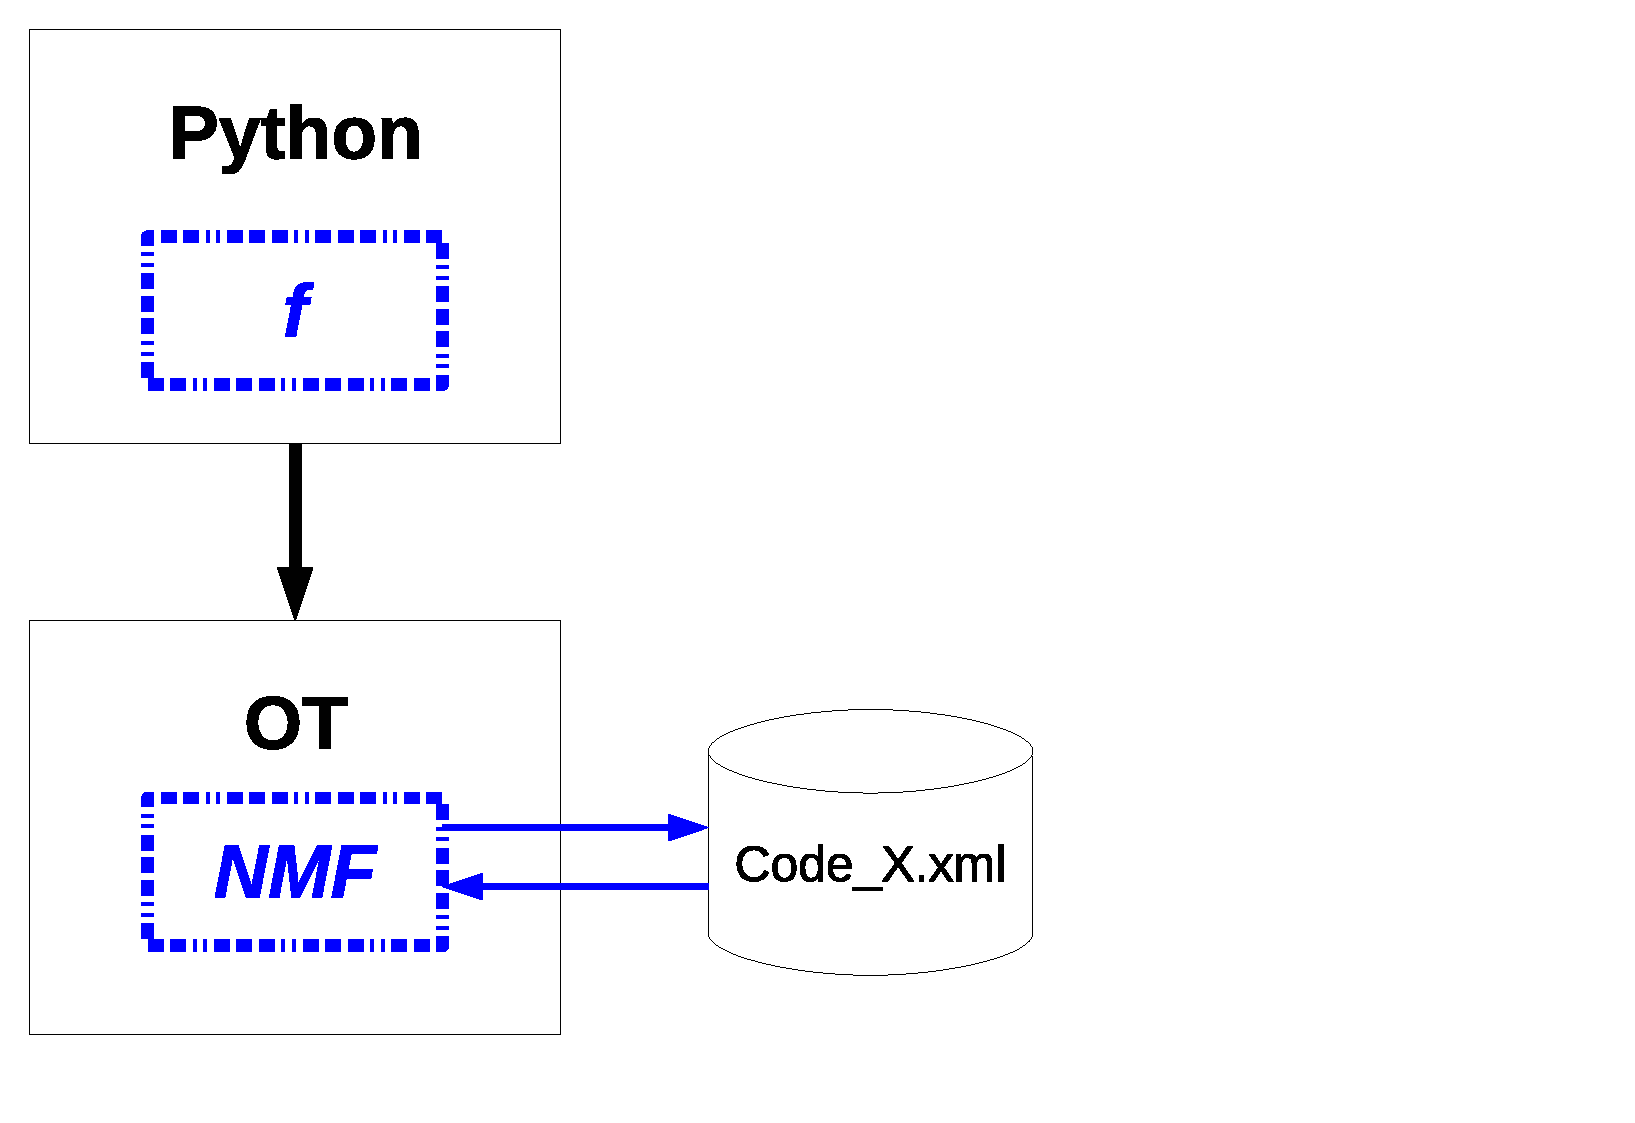
\includegraphics[width=12cm]{Figure4.pdf}
    \else
    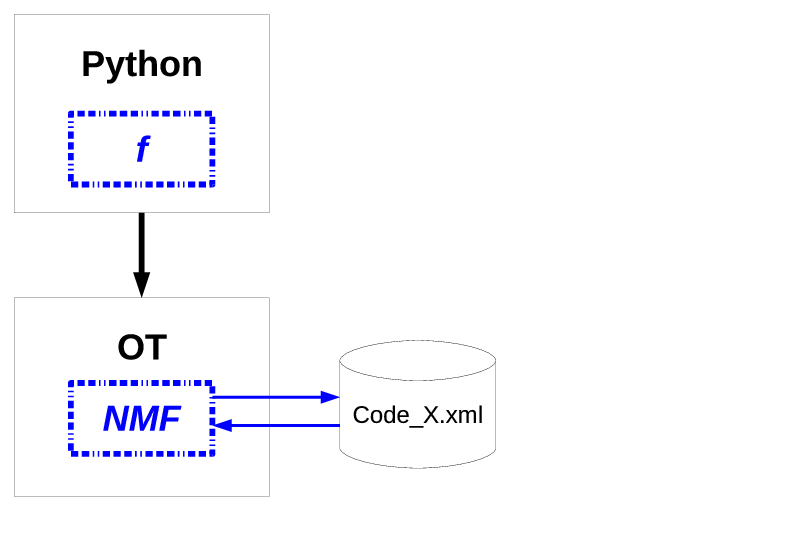
\includegraphics[width=12cm]{Figure4.png}
    \fi
    \caption[Figure 4]{Search of the \index{wrapper}wrapper's \index{description file}description file}
  \end{center}
\end{figure}

\subsubsection{Step 3: Analysis of the \index{description file}description file}

However, if the file is present, it is read. Any reading error causes a program error and the {\bf f} is not created. The details of this \index{description file}description file will be discussed later but, at this stage, it suffices to know that it contains the path to the {\bf Code\_X.so} \index{dynamic library}dynamic library (see Figure 3.5).

\begin{figure}
  \begin{center}
    \ifpdf
    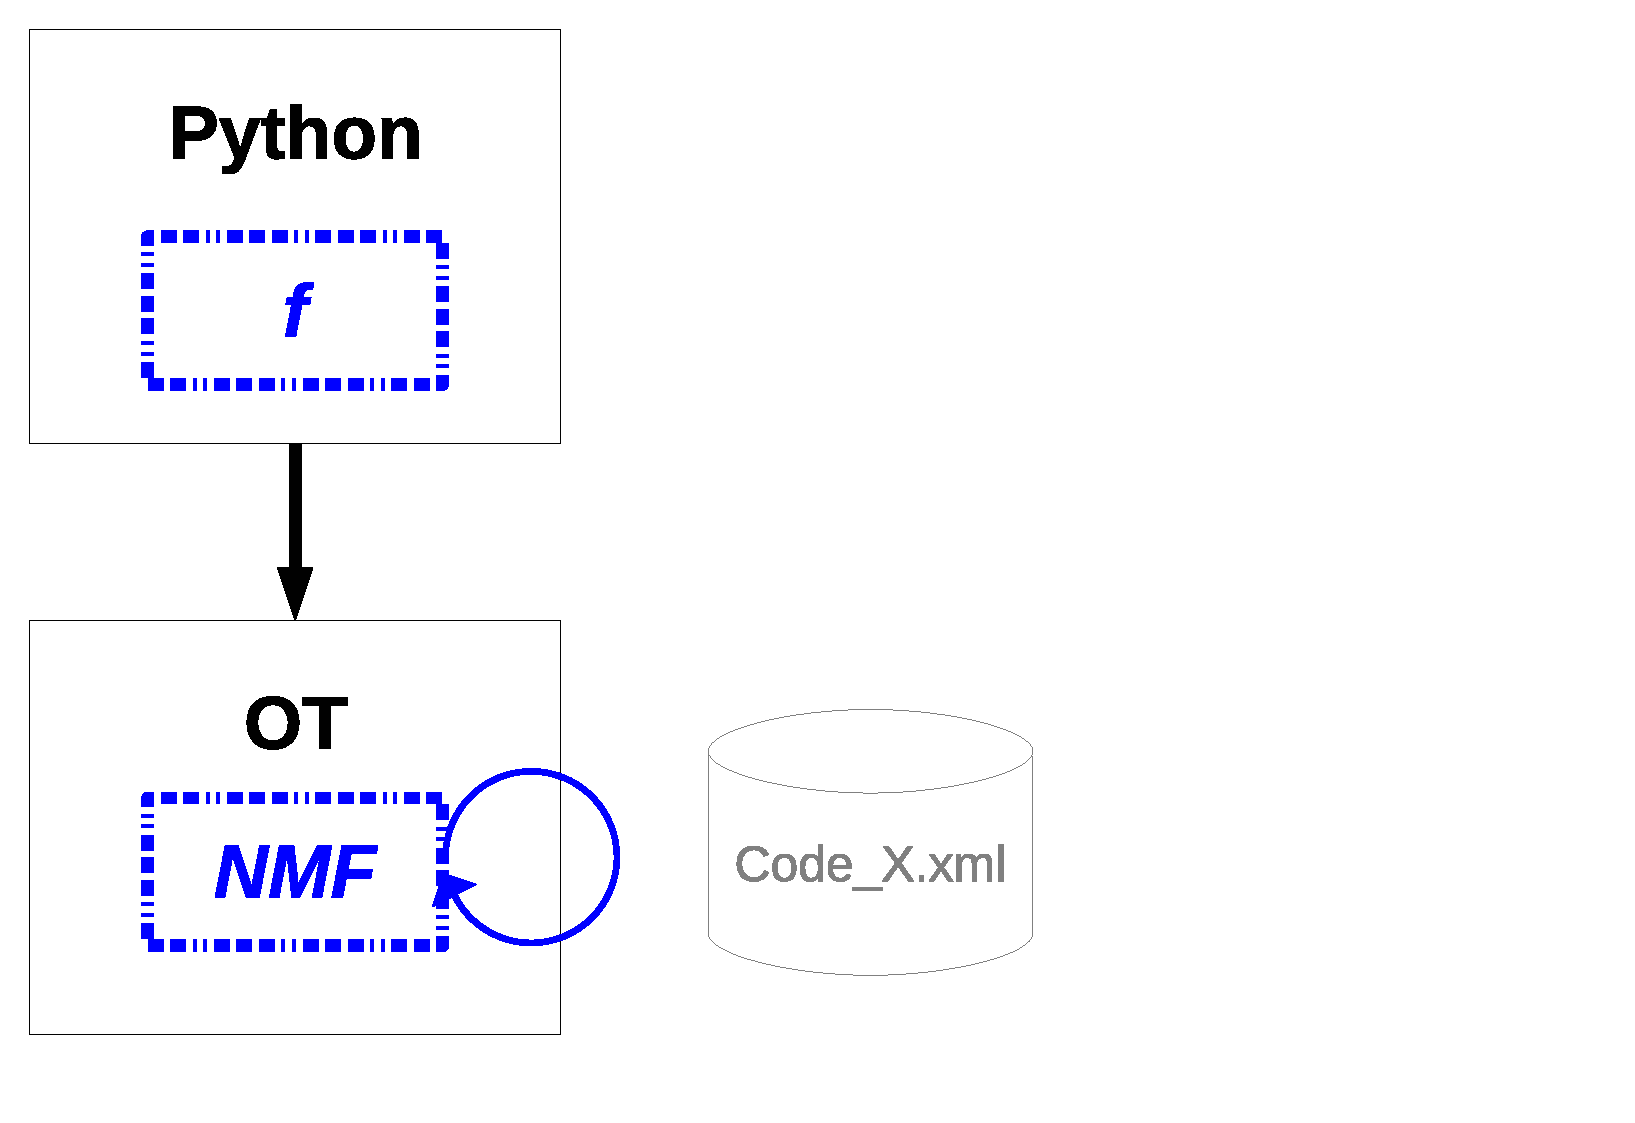
\includegraphics[width=12cm]{Figure5.pdf}
    \else
    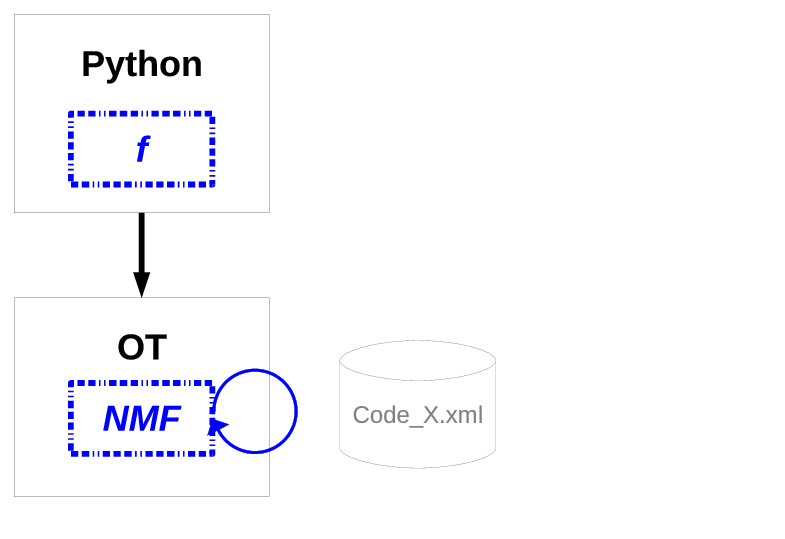
\includegraphics[width=12cm]{Figure5.png}
    \fi
    \caption[Figure 5]{Reading and analysis of the \index{wrapper}wrapper's \index{description file}description file}
  \end{center}
\end{figure}

\subsubsection{Step 4: Search for the \index{dynamic library}dynamic library}

In turn, this library will be searched for in the same directories. If it is found, it is automatically loaded by \OT (see Figure 3.6). Its absence causes an error.

\begin{figure}
  \begin{center}
    \ifpdf
    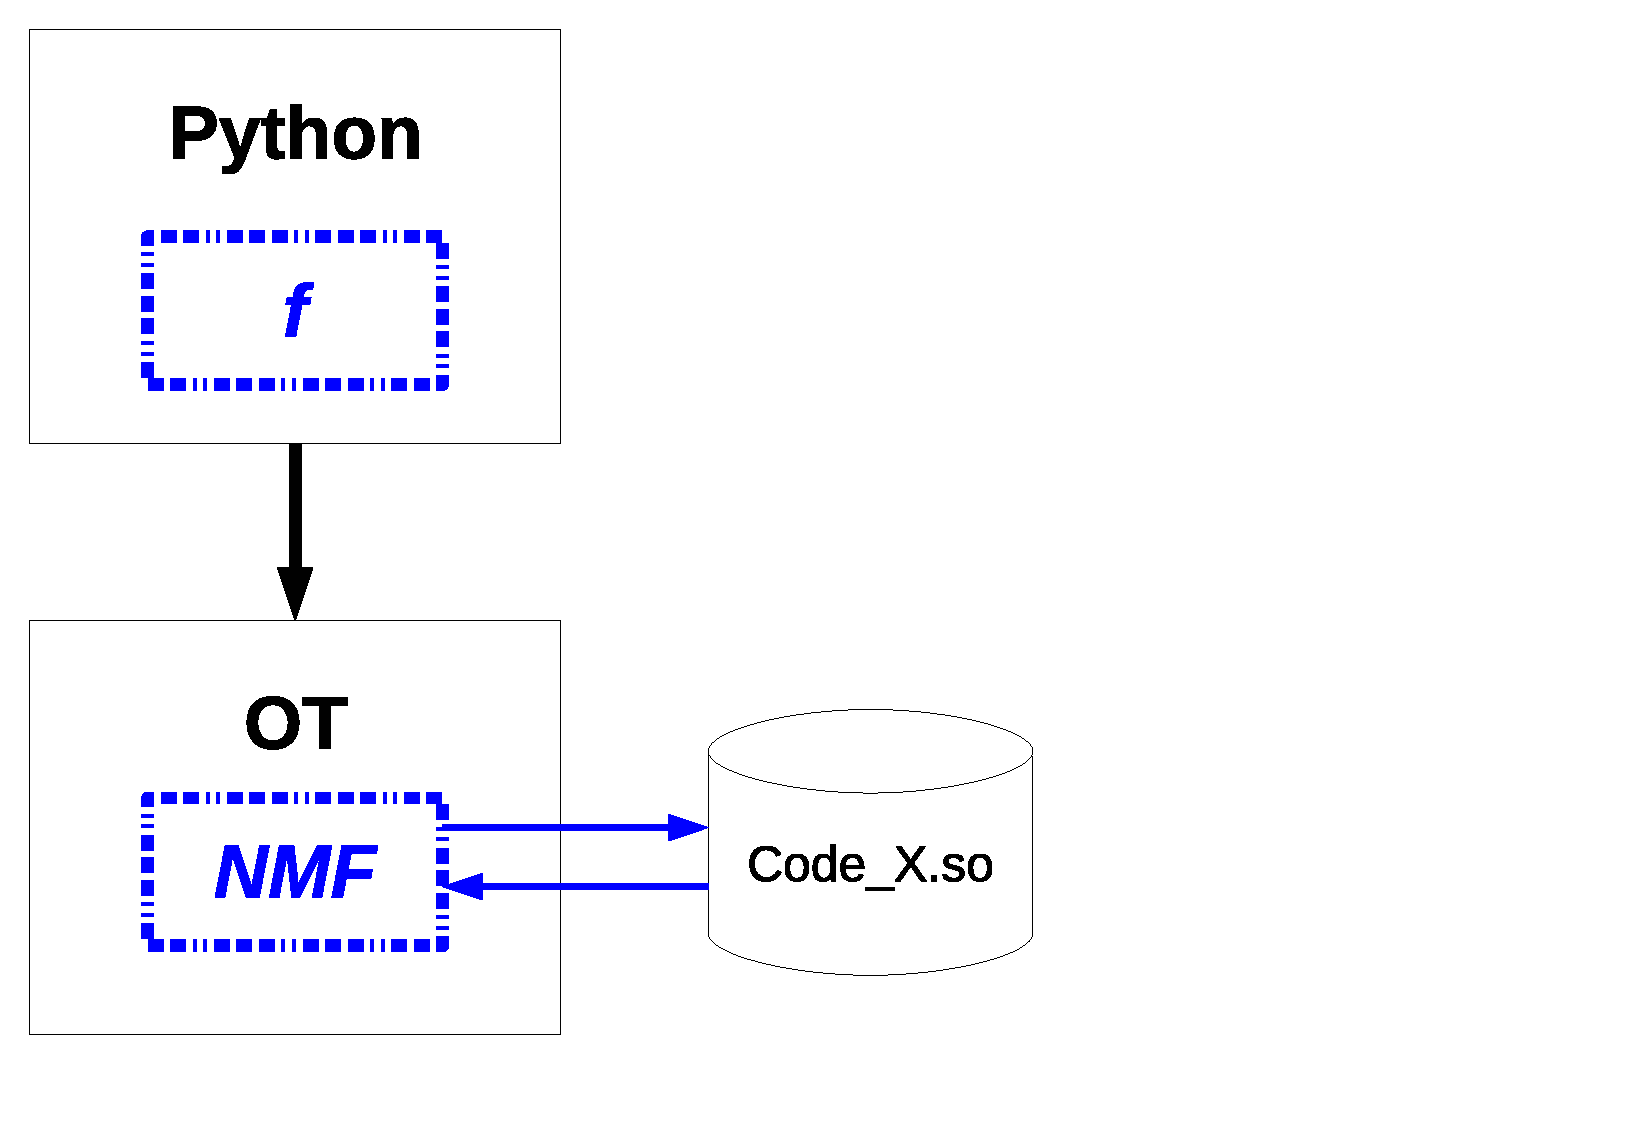
\includegraphics[width=12cm]{Figure6.pdf}
    \else
    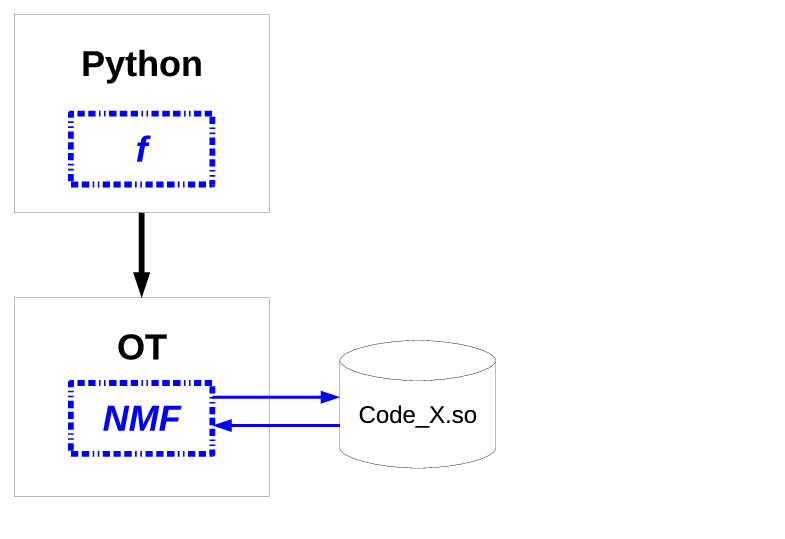
\includegraphics[width=12cm]{Figure6.png}
    \fi
    \caption[Figure 6]{Search for the \index{wrapper}wrapper's \index{dynamic library}dynamic library}
  \end{center}
\end{figure}

\subsubsection{Step 5: Loading the \index{dynamic library}dynamic library}

Once the library is loaded, it is tested to uncover some of its characteristics (see Figure 3.7). We will detail this \index{data structure}point in section 4.4.3, which deals with the {\bf getInfo\_}\footnote{At this stage of the document, the real names of the wrapper's functions have not been described yet. In fact, the \index{central term}{\bf getInfo\_} method carries a more elaborate name, with other elements as prefixes and suffixes. This will be described later on in the document. We will use the shortened name in order to simplify the text, as long as it does not raise any ambiguity.} method.

\begin{figure}
  \begin{center}
    \ifpdf
    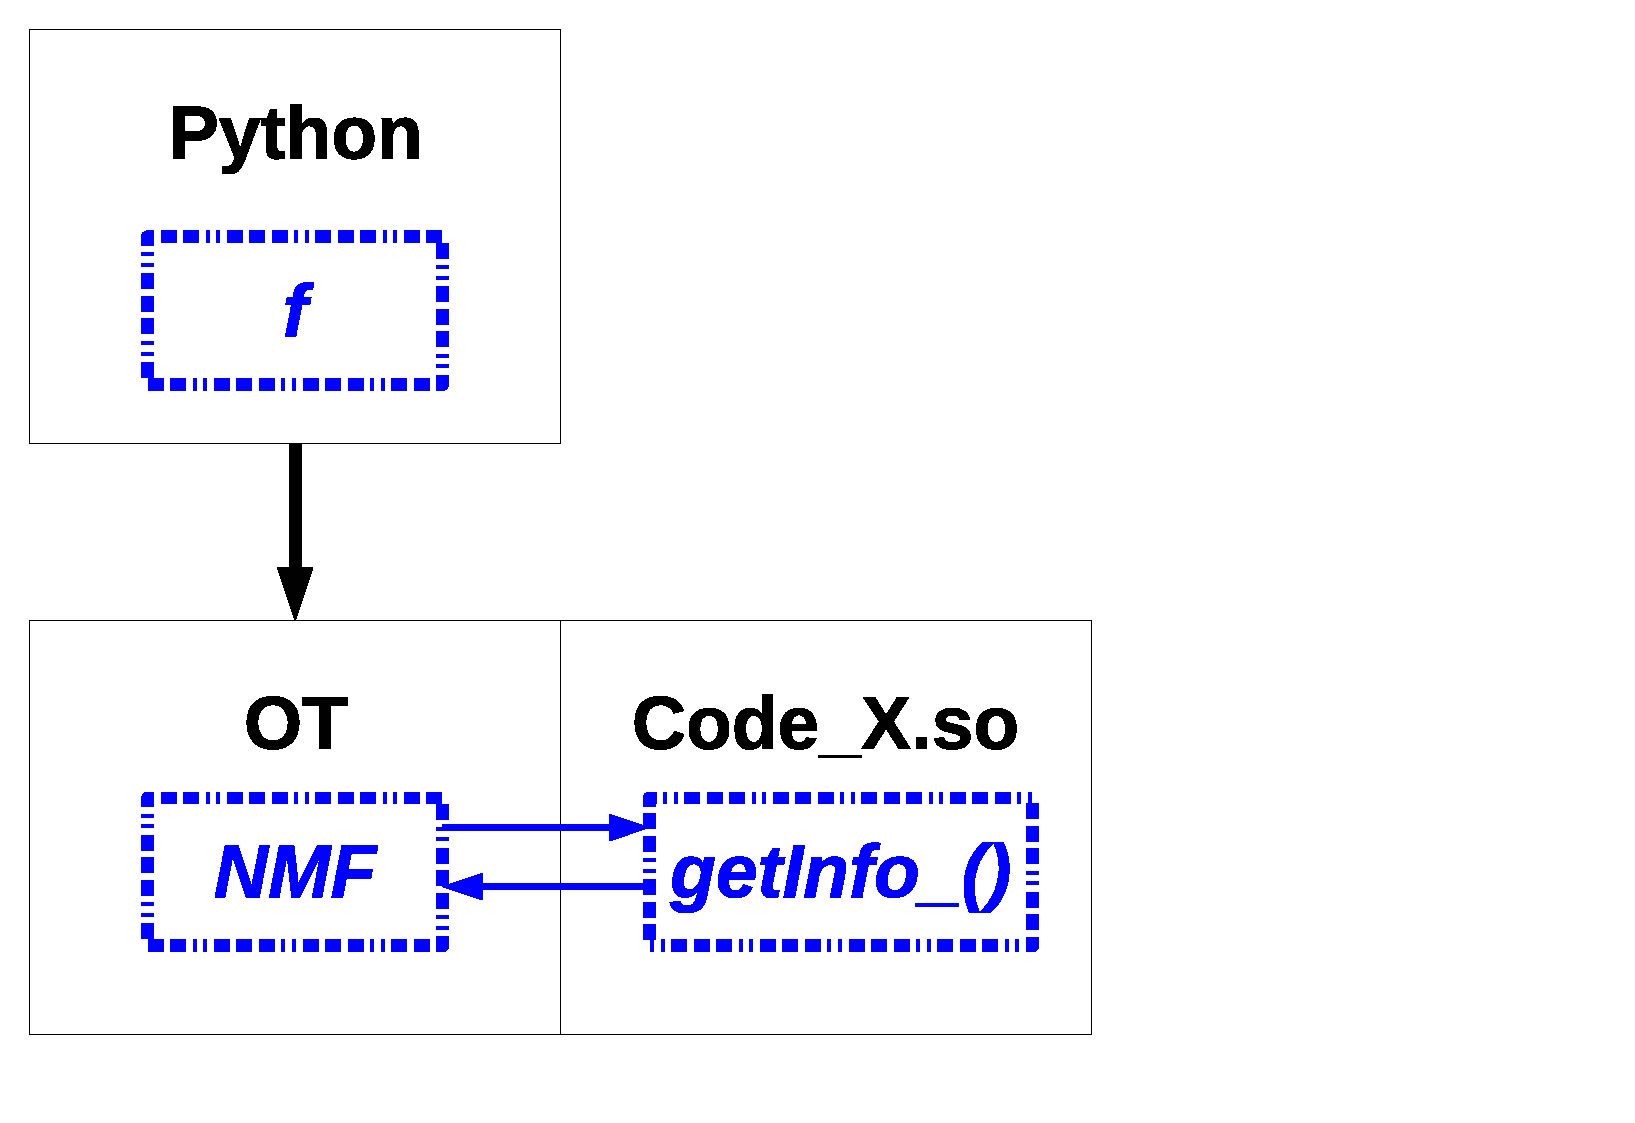
\includegraphics[width=12cm]{Figure7.pdf}
    \else
    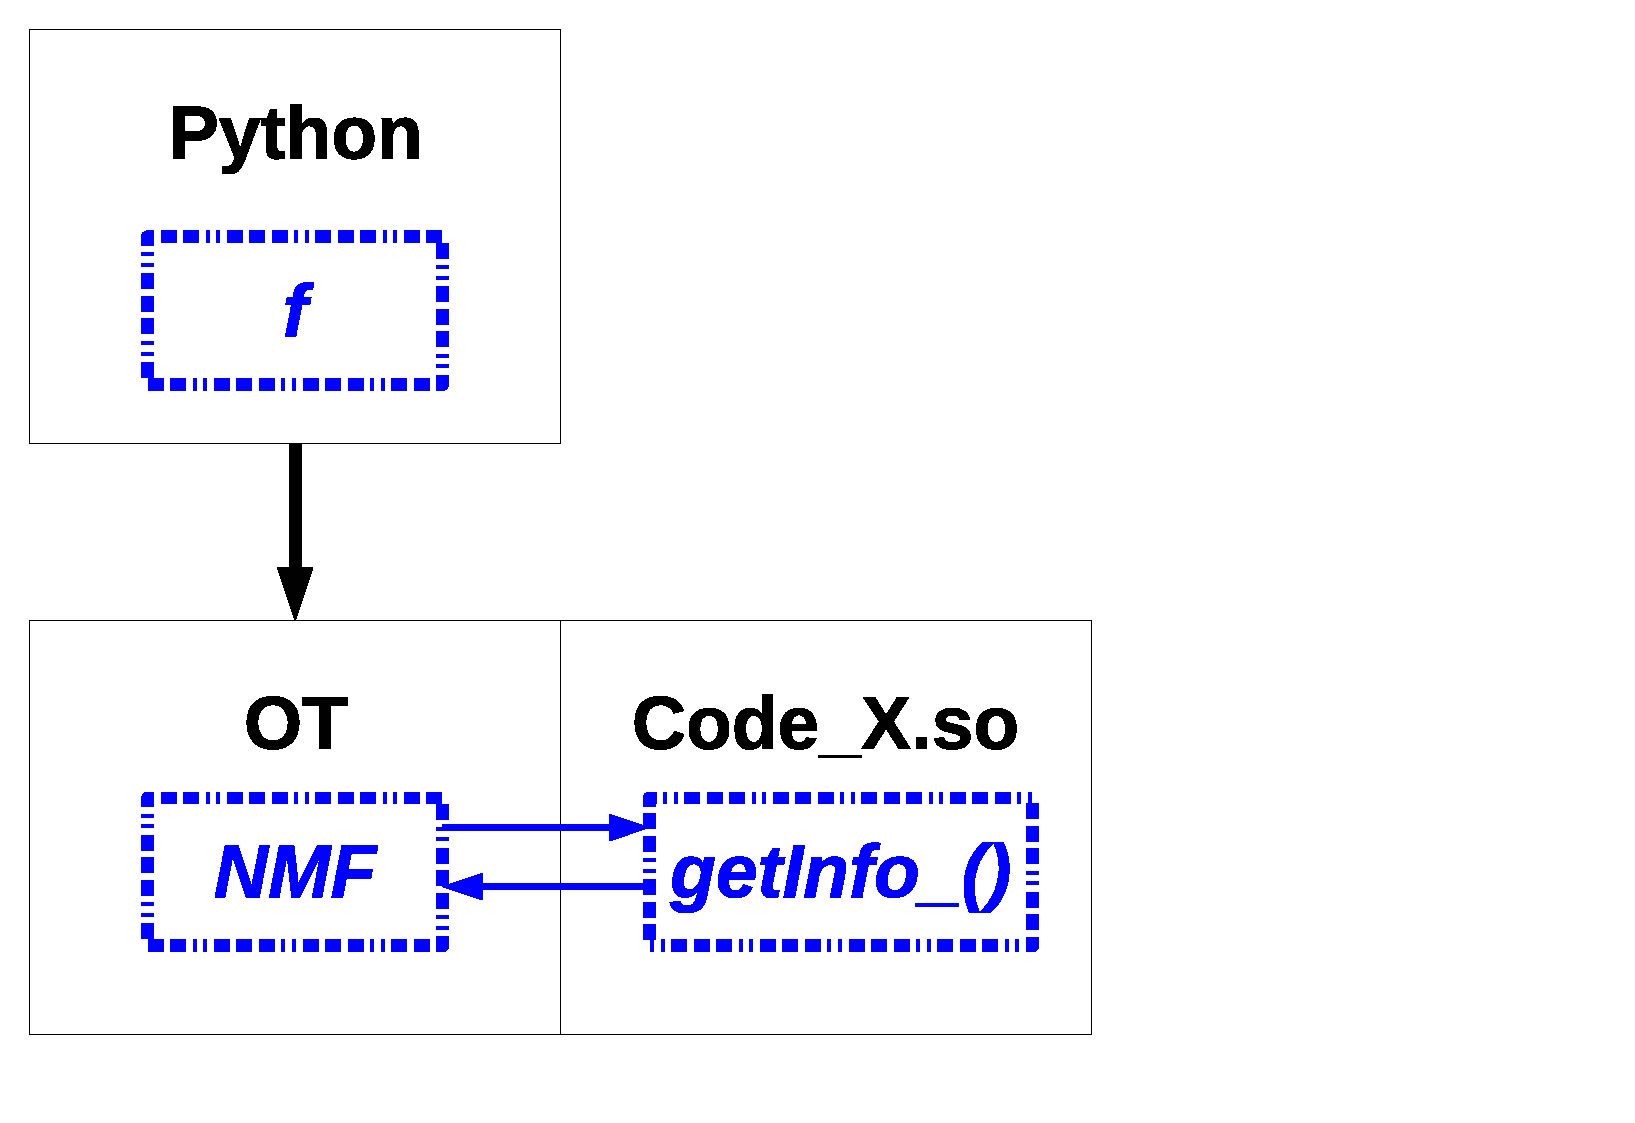
\includegraphics[width=12cm]{Figure7.pdf}
    \fi
    \caption[Figure 7]{Loading and querying the \index{dynamic library}dynamic library}
  \end{center}
\end{figure}

\subsubsection{Step 6: Completion of the \index{NumericalMathFunction}NumericalMathFunction construction}

Finally, \OT\ maintains an internal link to the \index{wrapper}wrapper's \index{dynamic library}dynamic library and returns a properly constructed and initialized \index{NumericalMathFunction}NumericalMathFunction object to the user (see Figure 3.8). It is therefore possible to use it for the study of uncertainties.

\begin{figure}
  \begin{center}
    \ifpdf
    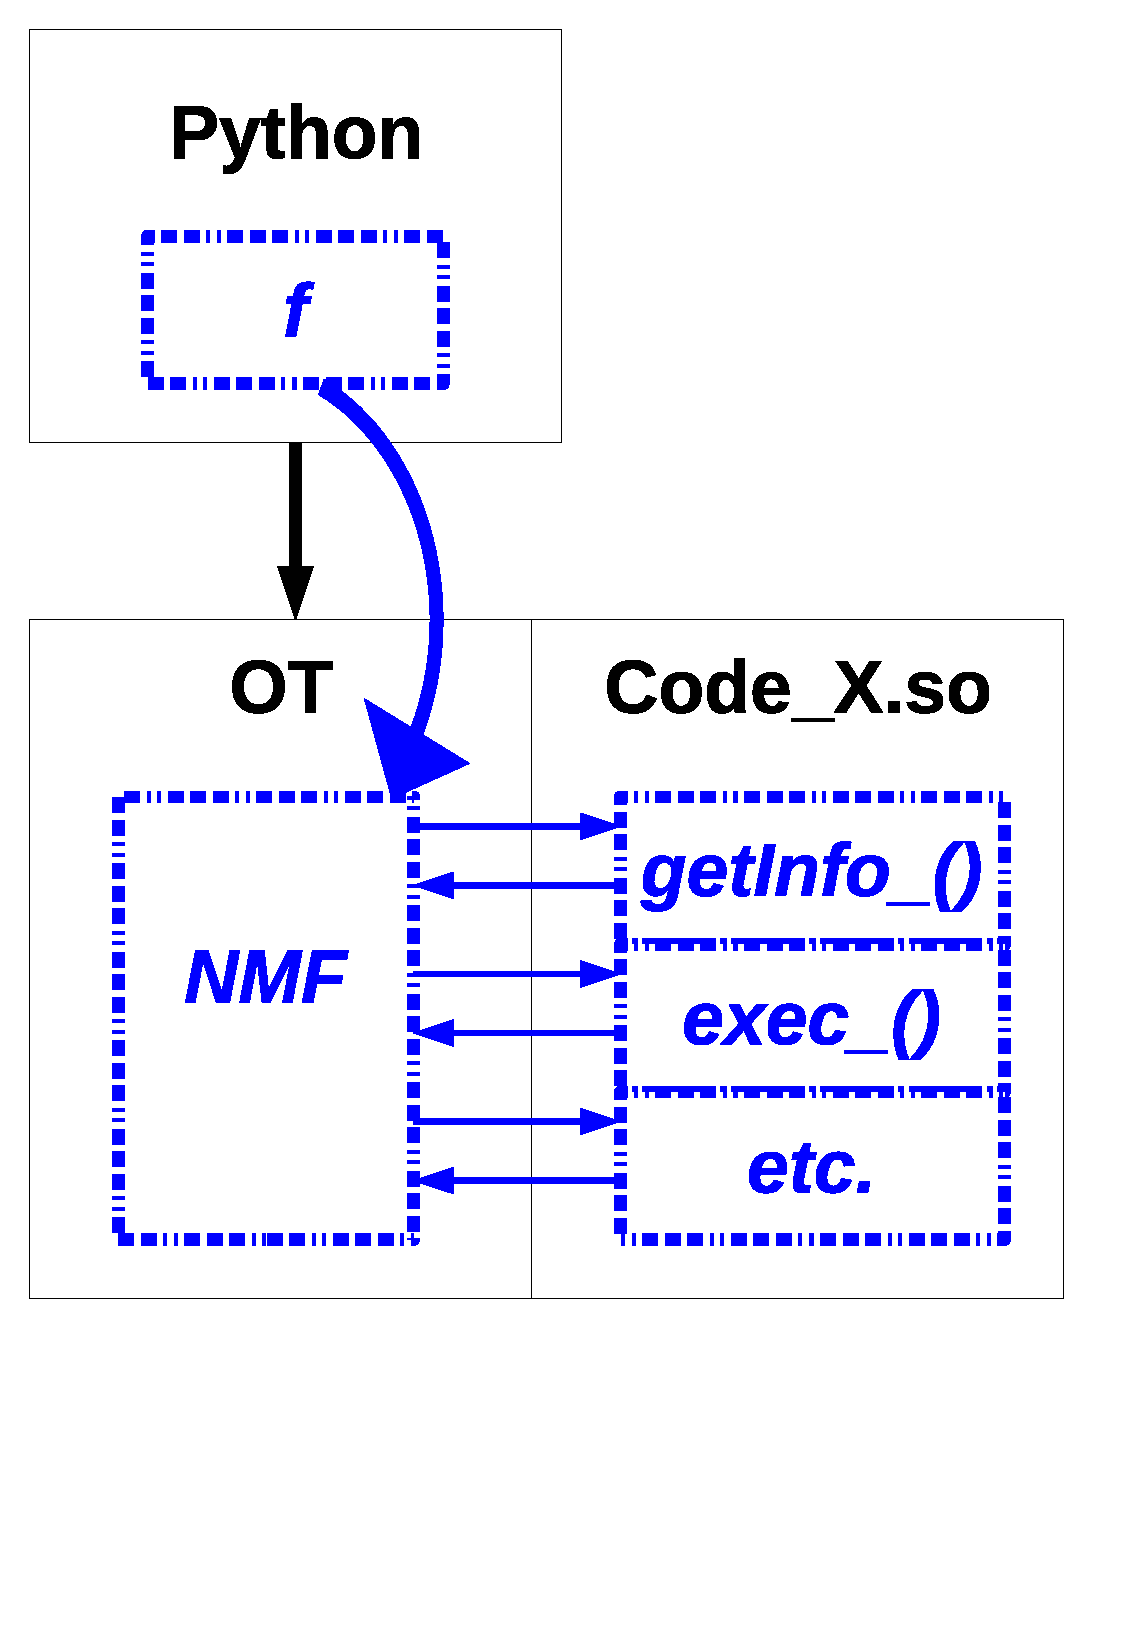
\includegraphics[height=12cm]{Figure8.pdf}
    \else
    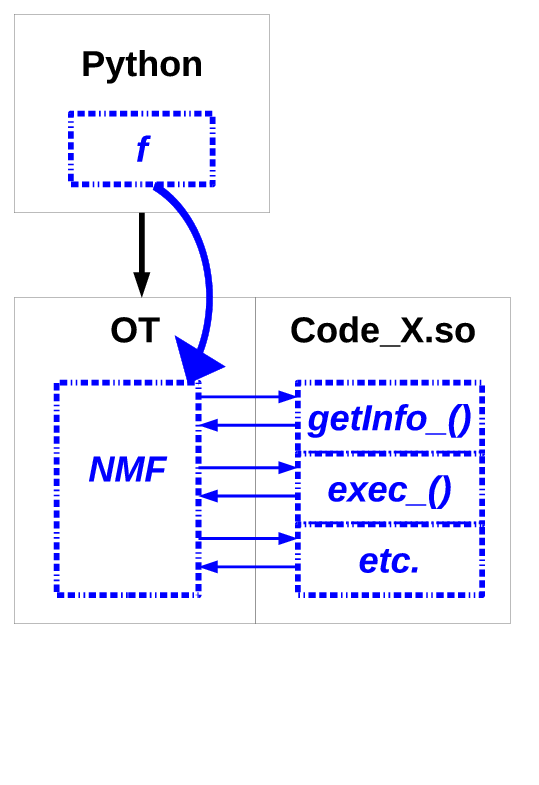
\includegraphics[height=12cm]{Figure8.png}
    \fi
    \caption[Figure 8]{Completion of the \index{NumericalMathFunction}NumericalMathFunction construction}
  \end{center}
\end{figure}

\subsection{Example: Creating a minimal \index{wrapper}wrapper}

To make this document more concrete, this section shows how to create a "minimal" \index{wrapper}wrapper. It will allow to browse the \index{description file}description file (see Section 3.2.4) and the source code in detail (see Section 3.2.5). It will especially help distinguish the elements that \emph{must} be present within any wrapper from elements that are optional and are only enriching features.

\subsubsection{Required Items}

In order not to unnecessarily complicate this first example, we will limit the \index{Function}Function implemented in the \index{wrapper}wrapper to a simple $\R^{3} \to \R^{2}$ analytical formula:

$$P\:\left\{\begin{array}{l}
    y_1 = x_1 \times e^{(- x_2 \times x_2)} \\
    y_2 = x_2 + x_3
  \end{array}\right.$$

We call this \index{Function}Function {\bf P}.

This \index{Function}Function is currently implemented directly in the \index{wrapper source code}source code of the \index{wrapper}wrapper. Later examples will show how this function can be extracted from the wrapper's body into an external code.

To create a \index{wrapper}wrapper based on {\bf P} which can be used by \OT, it is necessary to provide the library with the following elements:
\begin{itemize}
\item the path to the shared library that implements {\bf P}, {\bf P.so};
\item the list and description of variables exchanged between the \index{wrapper}wrapper and \OT, namely input variables ($x_1$, $x_2$ and $x_3$) and output variables ($y_1$ and $y_2$) of the \index{Function}Function;
\item the names of the \index{Function}Function within the \index{wrapper}wrapper, here {\bf P}, because the same wrapper can technically implement multiple Functions;
\item the name of the \index{Gradient}Gradient or the \index{Hessian}Hessian, if they are present in the \index{wrapper}wrapper, associated with the \index{Function}Function;
\item information on how P is implemented in the \index{wrapper}wrapper.
\end{itemize}

In our example, we will provide neither the \index{Gradient}Gradient nor the \index{Hessian}Hessian for {\bf P}, although this is quite feasible since P is very simple to derive. We will see later that the \OT\ library adapts itself and produces on its own a Gradient and a Hessian with centered finite differences.

\subsubsection{Starting from a template to generate the \index{wrapper}wrapper}

It is not easy, for a wrapper designer, to produce a first functional draft based on the analytical formula alone. Therefore, all versions of \OT\ offer by default a completely independent structure for wrapper development that allows to easily produce a wrapper.

Several development structures are offered in order to replace the old structure. The new structures are now available in the {\bf share/openturns/WrapperTemplates/<wrapper\_example>} subdirectory, where {\bf \index{wrapper}<wrapper\_example>} can be:
\begin{itemize}
\item {\bf wrapper\_calling\_shell\_command}: structure for the development of a wrapper launching the external code via a shell command line;
\item {\bf wrapper\_linked\_with\_C\_function}: structure for the development of a wrapper calling a C \index{function}function;
\item {\bf wrapper\_linked\_with\_F77\_function}: structure for the development of a wrapper calling a \index{FORTRAN}FORTRAN 77 \index{function}function.
\end{itemize}

We copy the {\bf \index{wrapper}wrapper\_linked\_with\_C\_function directory} as {\bf Pwrapper}:

\index{installation directory}
\lstset{language=Bash, basicstyle=\normalsize}
\begin{lstlisting}[frame=TBRL]
  > cp -r <openturns_dir>/share/openturns/WrapperTemplates/wrapper_linked_with_C
  _function $HOME/Pwrapper
\end{lstlisting}

Then, just use the {\bf customize} script which automatically renames the files with the name passed as an argument:

\lstset{language=Bash, basicstyle=\normalsize}
\begin{lstlisting}[frame=TBRL]
  > ./customize P
\end{lstlisting}

\subsubsection{Compilation and \index{installation}installation of the \index{wrapper}wrapper}

Before going into detail on how to write the wrapper, we need to prepare the development environment which will conduct the \index{compilation}compilation and installation of the library and of its XML file.

\small
\begin{quote}
  \textit{Note: To be able to use the {\bf Pwrapper} user development directory, the developer must have access to three GNU Open Source tools known as {\bf autoconf}, {\bf automake} and {\bf libtool}. These tools are commonly installed on all GNU/Linux distributions. However the installed versions may be older and it is always good to have the latest available update\footnote{See the website {\bf http://www.openturns.org} to check the tool versions adapted to the \OT\ version you are using.}.\\
    The user must also have a C or C++ compiler in order to produce the \index{wrapper}wrapper's \index{dynamic library}dynamic library. The GNU Open Source compiler {\bf gcc} is a very good choice.}
\end{quote}
\normalsize

The first step is to bootstrap the environment. To this end, the following command must be executed once:

\lstset{language=Bash, basicstyle=\normalsize}
\begin{lstlisting}[frame=TBRL]
  > bootstrap
\end{lstlisting}

Then we determine which tools are available on the computer in order to compile and install the \index{wrapper}wrapper. This configuration step is also carried out only once:

\index{installation directory}
\lstset{language=Bash, basicstyle=\normalsize}
\begin{lstlisting}[frame=TBRL]
  > ./configure --with-openturns=<openturns_dir>
\end{lstlisting}

By default, the \index{wrapper}wrapper is installed in the directory {\bf \$HOME/openturns/wrappers} which is a standard search directory of \OT.

\small
\begin{quote}
  \textit{Note: If the wrapper must be installed in a different directory, it is necessary to use the option {\bf --prefix = <Pwrapper\_dir>} where {\bf <Pwrapper\_dir>} is the directory where the wrapper will be installed (later on). When using the wrapper, the path to {\bf <Pwrapper\_dir>} should be positioned in the environment variable \index{wrapper search}{\bf OPENTURNS\_WRAPPER\_PATH}.}
\end{quote}
\normalsize

When the source files needed to produce the \index{wrapper}wrapper are written (see sections 3.2.4 and 3.2.5), it will be possible to compile and then install the wrapper using the commands:

\lstset{language=Bash, basicstyle=\normalsize}
\begin{lstlisting}[frame=TBRL]
  > make
  > make install
\end{lstlisting}

\subsubsection{\index{description file}Description file for the minimal \index{wrapper}wrapper}

We begin by writing, or rather by modifying the description file {\bf P.xml}.

This XML file is highly structured and must contain a certain number of tags. This rigid syntax is checked by a grammar (\index{DTD}DTD) described in the \index{wrapper}{\bf wrapper.dtd} file. This DTD is provided by default by \OT\footnote{The file should normally be found in the {\bf <openturns\_dir>/share/openturns/wrappers} directory.}. Any error in the syntax or the structure of the XML file results in immediate rejection by the \OT\ library and prevents from loading the wrapper.

The {\bf P.xml} file contains the following tags:

\begin{description}
\item[<wrapper>] \index{wrapper}This tag introduces the general description of the wrapper.

\item[<library>] This tag introduces the section dealing with the \index{dynamic library}dynamic library as seen from the \OT standpoint.

\item[<path>] This tag allows to indicate to \OT\ where to find the wrapper's dynamic library, {\bf P.so} in our convention. It thus reads:

  \lstset{language=XML, basicstyle=\normalsize}
  \begin{lstlisting}[frame=TBRL]
    <wrapper>
    <library>
    <path>P.so</path>
    ...
  \end{lstlisting}

  The name of the \index{dynamic library}dynamic library is marked by the opening tag {\bf <path>} and the closing tag {\bf </path>} following the standard XML syntax. Be careful not to introduce whitespaces or any other separator, for all characters between the opening and closing tags \emph{will} be considered as the library name. The library will be sought in the same directory as the XML file (see Section 3.1.3) because the system assumes that both files are placed in the same directory.

  If the library name is preceded by a relative path, this path will be relative to the above-mentioned search directories. Absolute paths are relative to the computer's file system.

\item[<description>] This tag introduces the definition of the \index{Function}Function, the \index{Gradient}Gradient, the \index{Hessian}Hessian and of the exchanged variables.

\item[<variable-list>] This tag introduces the list of input and output variables of the \index{wrapper}wrapper.

\item[<variable>] This tag allows to define a wrapper input or output variable  as shown in the following example.

  \lstset{language=XML, basicstyle=\normalsize}
  \begin{lstlisting}[frame=TBRL]
    ...
    <description>
    <variable-list>

    <!-- three input variables -->
    <variable id="x1" type="in" />
    <variable id="x2" type="in" />
    <variable id="x3" type="in" />

    <!-- two output variables -->
    <variable id="y1" type="out" />
    <variable id="y2" type="out" />

    </variable-list>
    ...
  \end{lstlisting}

  It is used to declare the three input variables ({\bf x1}, {\bf x2} and {\bf x3}) and two output variables ({\bf y1} and {\bf y2}) of the {\bf P} \index{Function}Function. The {\bf id} attribute specifies the variable name and the {\bf type} attribute, its nature ({\bf in} for input and {\bf out} for output, from the point of view of {\bf P}). We remind here that the exchanged variables are doubles.

  It is a good practice to list the variables in their natural order, input before output. This order is used internally by \OT\ so as to determine to which variable it must assign the values of the input and output point components when evaluating the Function. Thus, the first component of the point\index{data structure} will be assigned to the first listed variable, the second component to the second listed variable, and so on.

  Each variable must have a unique identifier ({\bf id}). If this is not the case, the \index{description file}description file is rejected.

  We will see later on that the {\bf <variable>} tags may be supplemented by sub-tags providing additional information.

\item[<function>, <gradient>, <hessian>] These three tags are used to respectively define the names of the \index{Function}Function, the \index{Gradient}Gradient and the \index{Hessian}Hessian. In our example of a minimal \index{wrapper}wrapper, only the Function is defined under the name {\bf P}. The name is written between the opening and closing tags without spaces or any other superfluous character.

  \lstset{language=XML, basicstyle=\normalsize}
  \begin{lstlisting}[frame=TBRL]
    ...
    <function provided="yes">P</function>
    <gradient provided="no" />
    <hessian  provided="no" />
    </description>
    </library>
    ...
  \end{lstlisting}

  The {\bf <function>}, {\bf <gradient>} or {\bf <hessian>} tags include a {\bf provided} attribute that indicates whether the Function, the Gradient or the Hessian is implemented in the wrapper ({\bf yes}) or not ({\bf no}). In the latter case, the name need not be specified.

\item[<external-code>] This tag introduces the definition of the coupling between the wrapper and the external code.

\item[<data>] This tag introduces the definition of the data exchanged between the wrapper and the external code. In our minimal example, there really is no external code since the wrapper will play this role without resorting to some other object. This section will therefore remain empty.
\end{description}

The remaining information to be given to \OT\ deals with the way the \index{wrapper}wrapper internally implements the \index{Function}Function. The presence of this information is justified for the development of a generic wrapper, but is useless in the example at hand. Yet it is still necessary to provide these pieces of information in order to have a valid \index{description file}description file. Future developments of \OT\ will eliminate this dependence.

\begin{description}
\item[<wrap-mode>] This tag indicates the way the \index{wrapper}wrapper internally implements the \index{Function}Function.

  The {\bf type} attribute indicates that the Function is directly coded within the wrapper ({\bf static-link}). The sub-tags {\bf <in-data-transfer>} and {\bf<out-data-transfer>} specify that the variables must be passed to the Function as arguments.

\item[<command>] This tag describes the system command that calls the external code when it is fully independent and disjoint from the wrapper. Here, since the wrapper is minimal, no command is defined.

  \lstset{language=XML, basicstyle=\normalsize}
  \begin{lstlisting}[frame=TBRL]
    ...
    <external-code>
    <data />

    <wrap-mode type="static-link">
    <in-data-transfer  mode="arguments" />
    <out-data-transfer mode="arguments" />
    </wrap-mode>

    <command />

    </external-code>
    </wrapper>
  \end{lstlisting}
\end{description}

Finally, the \index{description file}description file {\bf P.xml.in} for our minimal \index{wrapper}wrapper looks like this:\index{DTD}
\lstset{language=XML, basicstyle=\normalsize}
\begin{lstlisting}[frame=TBRL]
  <?xml version="1.0" encoding="ISO-8859-1"?>
  <!DOCTYPE wrapper SYSTEM "@OPENTURNS_WRAPPER_DTD_PATH@/wrapper.dtd">

  <wrapper>
  <library>
  <path>P.so</path>
  <description>
  <variable-list>
  <variable id="x1" type="in"  />
  <variable id="x2" type="in"  />
  <variable id="x3" type="in"  />
  <variable id="y1" type="out" />
  <variable id="y2" type="out" />
  </variable-list>
  <function provided="yes">P</function>
  <gradient provided="no" />
  <hessian  provided="no" />
  </description>
  </library>
  <external-code>
  <data />
  <wrap-mode type="static-link">
  <in-data-transfer  mode="arguments" />
  <out-data-transfer mode="arguments" />
  </wrap-mode>
  <command />
  </external-code>
  </wrapper>
\end{lstlisting}

\subsubsection{Source code for the minimal \index{wrapper source code}wrapper}

The second file needed to produce the \index{wrapper}wrapper is the source code of the \index{dynamic library}dynamic library ({\bf wrapper.c}).

This source code is used to carry out the interface adaptation required by the data transfer between \OT\ and the \index{Function}Function to implement. It could theoretically be written in any language evolved enough to perform such operations. But the fact that the \index{wrapper}wrapper's library is dynamically loaded, and that \OT\ must search for symbols in it and be able to call them, requires the use of a computer interface based on C. This sets strong constraints on the languages that can be used to code the wrapper. Only C and C++ are easily usable for this task.

\small
\begin{quote}
  \textit{Note: This constraint does not mean that the developer should be a C or C++ expert to be able to develop a wrapper. The engineering work done in \OT\ helped greatly simplify the writing of the wrapper, and any developer used to a procedural language (\index{FORTRAN}FORTRAN or other) is able to generate a wrapper. However, they must obey the rules imposed by \OT.}
\end{quote}
\normalsize

The first thing to do, in the \index{wrapper source code}source file {\bf wrapper.c}, is to include the header file which provides definitions needed for \index{compilation}compilation:\index{Wrapper.h}

\lstset{language=C, basicstyle=\normalsize}
\begin{lstlisting}[frame=TBRL]
  #include "Wrapper.h"
  ...
\end{lstlisting}

These two files are provided by default in the \OT\ \index{installation}installation.

The file {\bf Wrapper.h} is absolutely essential and should always be included in the source code of the wrapper. It gathers all the definitions that allow communication between the \OT\ library and the wrapper. Without this file, no compilation of the wrapper is possible.

It also contains the declarations of functions that are practical and shared by many wrappers. These functions are part of the platform with which the wrapper connects itself. The use of these functions greatly simplifies the writing of wrappers by performing the most common actions in a simple and efficient way. This documentation largely relies on them. The first appendix describes the functions in this library.

Let's recall the definition of our {\bf P} \index{Function}Function:

$$P\:\left\{\begin{array}{l}
    y_1 = x_1 \times e^{(- x_2 \times x_2)} \\
    y_2 = x_2 + x_3
  \end{array}\right.$$

Among the different techniques available to implement the {\bf P} Function in the \index{wrapper}wrapper, we choose to isolate the computation in a separate C \index{function}function which we call {\bf myP}. The function being multidimensional $\R^{3} \to \R^{2}$, the C function has been designed to accept an array of 3 doubles as input and an array of 2 doubles as output.

We assume that the arrays are already allocated with the proper size (respectively $n$ and $p$) and that only the output values are to be modified.

We also use the C function return value to indicate a possible miscalculation. Here, since the calculation is always possible, the function systematically returns 0 to indicate that no error occurred (this is a C convention). In case of an error, such as a division by zero or an argument outside the Function's definition domain, the function needs to return a non-zero return code.

\lstset{language=C, basicstyle=\normalsize}
\begin{lstlisting}[frame=TBRL]
  ...
  #include <math.h>

  int myP ( double * x, unsigned long n,
  double * y, unsigned long p )
  {
    y[0] = x[0] * exp( - x[1] * x[1] );
    y[1] = x[1] + x[2];
    return 0;
  }
  ...
\end{lstlisting}

In the example, we used the names {\bf x} and {\bf y} to refer to the input variables ({\bf x1}, {\bf x2} and {\bf x3}) and output variables ({\bf y1} and {\bf y2}). However, seing that the C language requires to start numbering array indices from zero: {\bf x[0]} corresponds to {\bf x1}, {\bf x[1]} to {\bf x2}, etc.

\small
\begin{quote}
  \textit{Note: Inclusion of the {\bf math.h} file is justified by the use of the {\bf exp} \index{function}function.}
\end{quote}
\normalsize

Having this {\bf P} \index{Function}Function, we now need to interface it with \OT. This is done using an auxiliary \index{function}function that will ensure communication with the \OT\ library.

This function is commonly called \index{central term}{\bf exec\_}, although its name is more complex as shown by the following example:

\index{prefix}\index{internal state}\index{data structure}
\lstset{language=C, basicstyle=\normalsize}
\begin{lstlisting}[frame=TBRL]
  ...
  enum WrapperErrorCode func_exec_P ( void * p_state,
  const struct point * inPoint,
  struct point * outPoint )
  {
    if ( myP (inPoint->data_,  inPoint->size_,
    outPoint->data_, outPoint->size_ ) ) return WRAPPER_EXECUTION_ERROR;

    return WRAPPER_OK;
  }
\end{lstlisting}

The \index{central term}{\bf exec\_} \index{function}function is responsible for calling the previously written {\bf myP} function and passing to it the ad-hoc arguments that it will search within the data structures passed as arguments. These data structures are already allocated and filled (for those who may be) so that the functions of the \index{wrapper}wrapper simply have to fill them. No memory management is to be performed at this level in the wrapper, which makes it very simple to use.

We have seen that the {\bf myP} \index{function}function could, in case of failure, warn the calling code about it. This case is treated by the test ({\bf if}) which returns a {\bf WRAPPER\_EXECUTION\_ERROR} error code to \OT. Otherwise the \index{return code}{\bf WRAPPER\_OK} code indicates that everything went smoothly.

\subsubsection{Checking if the minimal \index{wrapper}wrapper is functioning}

This being written, we saw that we only needed to compile and install the wrapper to run it (see sections 3.2.2 and 3.2.3). If the wrapper was installed in a standard \OT\ directory or if the \index{wrapper search}{\bf OPENTURNS\_WRAPPER\_PATH} environment variable was correctly set, it is possible to test its basic operation by using a small Python script (eg {\bf test\_P.py}) which is executed as follows:

\lstset{language=Bash, basicstyle=\normalsize}
\begin{lstlisting}[frame=TBRL]
  > python test_P.py
\end{lstlisting}

Congratulations! You have written the smallest possible wrapper and you have interfaced it with \OT.

After loading the entire \OT\ library ({\bf import}), the script creates a \index{NumericalMathFunction}NumericalMathFunction type object ({\bf P}) which loads the \index{wrapper}wrapper that we just built. It then evaluates this P object by passing a NumericalPoint ({\bf x}) to it as an argument. This action causes the \index{execution}execution of the C \index{function}function {\bf myP}, computing the analytical formula written in the source code of the \index{wrapper source code}wrapper, and the return of the value of the computed \index{NumericalMathFunction}NumericalPoint ({\bf y}).

Essentially, the script {\bf test\_P.py} carries out the following series of actions:

\lstset{language=Python, basicstyle=\normalsize}
\begin{lstlisting}[frame=TBRL]
  >>> from openturns import *
  >>> P = NumericalMathFunction ( "P" )
  >>> x = NumericalPoint ( 3 )
  >>> x[0] = 10.
  >>> x[1] = 20.
  >>> x[2] = 30.
  >>> print x
  [...]
  >>> y = P ( x )
  >>> print y
  [...]
\end{lstlisting}

\cleardoublepage

\section{The structure of a wrapper}
% Copyright (c)  2005-2009  EDF-EADS-PHIMECA.
% Permission is granted to copy, distribute and/or modify this document
% under the terms of the GNU Free Documentation License, Version 1.2
% or any later version published by the Free Software Foundation;
% with no Invariant Sections, no Front-Cover Texts, and no Back-Cover
% Texts.  A copy of the license is included in the section entitled "GNU
% Free Documentation License".

The rest of this document presents extensions to the mechanism described in the previous section, as well as the progressive externalization of the computation into an external code. Through these enhancements, we will see in detail the structure of the \index{wrapper}wrapper and the range of possibilities offered to the developer. If the example of the minimal wrapper allows to very quickly and easily test the interfacing of a formula with \OT , the techniques described in this section will guide the reader towards features of progressive difficulty. It is important to consider that these features are mostly optional and are mainly improvements to the interfacing of the computational code with \OT . Therefore, the developer can intentionally forget about them at first and start with a simple wrapper. The complexity will come later according to needs and developments of the computational code.

In short, the interfacing mechanism of a code with \OT\ is scalable and the developer only needs to produce the functions necessary for their code.

This touches one of the basic criteria that have guided the development of the tool: genericity. \OT\ has been designed as a tool that can interface with almost any computational code. But they can be very diverse and the wrapper for one code can be very different from the wrapper for another. Therefore, we had to invent a mechanism that satisfies both without excessively penalizing either one. This section will therefore lead us into considerations that the reader may, at first, see as complex or unnecessary. However, they are the result of specific requests for given codes. They are thus useful. Their complexity has been reduced as much as possible but it cannot always be hidden. The keyword for the reader here is to ignore what does not primarily concern them, in order keep the wrapper simple and suited to their needs.

\subsection{Naming conventions}

When the \OT\ platform loads the wrapper's \index{dynamic library}dynamic library ({\bf wrapper.so}), it is confronted to an object that it must identify as a code \index{wrapper}wrapper and, moreover, as the wrapper for the right computational code. It may happen that another software also uses a library called {\bf wrapper.so} and that this library be placed in an \OT\ search path, in which case the loading succeeds but the library is unusable. It is also possible that the {\bf wrapper.so} library is the wrapper for another code interfaced with \OT . This happens when developers do not change the name of the library to match the name of their code: everyone uses the same name.

In order to detect some of these cases and avoid unnecessary computations run on unwanted codes, it is necessary to allow \OT\ to check that the library being loaded is the expected one. This is done by requiring the wrapper to use names whose structure ensures (to some extent) an unambiguous identification.

\subsubsection{In the wrapper's source file}

The names of the proposed C functions are built on three elements:
\begin{itemize}
\item a \index{prefix}prefix ({\bf func\_}, {\bf grad\_} or {\bf hess\_}) that indicates whether the \index{function}function relates to the \index{Function}Function, the \index{Gradient}Gradient or the \index{Hessian}Hessian of the \index{NumericalMathFunction}NumericalMathFunction;
\item a \index{central term}central term which provides information on the treatment carried out by the C function; this will be detailed in Section 4.3;
\item a suffix that specifies what Function, Gradient or Hessian is actually implemented by the C function.
\end{itemize}

An example is more eloquent. Consider again what has been shown in section 3.2.5 on the \index{wrapper source code}wrapper's source code. We used two C functions named {\bf func\_getInfo\_P} and \index{execution}{\bf func\_exec\_P}. The name of the {\bf func\_getInfo\_P} function indicates that it informs \OT\ about the parameters ({\bf getInfo\_}) of the Function ({\bf func\_}) which implements the P Function ({\bf P}), while the {\bf func\_exec\_P} function name indicates that it carries out the computation ({\bf exec\_}) of the function ({\bf func\_}) which implements the P Function ({\bf P}).

We will see later that the \index{wrapper}wrapper is divided into three main parts, the \index{Function}Function, the \index{Gradient}Gradient and the \index{Hessian}Hessian, which are very similar. Each of these parts is further divided into C functions, whose number may vary. These functions are distinguished from each other by the \index{central term}central term, which describes their role within the section.

The introduction of the name of the Function, Gradient or Hessian as a suffix results from a dual intent. First of all, it allows to clearly identify the computation carried out by the \index{function}function and, therefore, to check that the loaded wrapper is the right one. It also allows to build a wrapper having multiple Functions, Gradients and Hessians in the same source code, in order to simultaneously have several implementations:
\begin{itemize}
\item of the same code, as is the case when an implementation is better than another, but both are useful, or that each implementation is used in different contexts; for example, each of them executes the code on a different machine or in a different version;
\item of different codes; one might want to put in the same wrapper implementations related to different codes but most often executed together, as is the case when one sets up couplings.
\end{itemize}

\subsubsection{In the \index{wrapper}wrapper's \index{description file}description file}

The name of the \index{Function}Function is introduced by the string given between the opening tag {\bf <function>} and the closing tag {\bf </function>} of the wrapper's description file. It is important to not insert any whitespace, blank or other separator in the name because it would prevent \OT\ from building a correct name and jeopardize the loading of the \index{dynamic library}dynamic library wrapper.

Symmetrically, the name of the \index{Gradient}Gradient or \index{Hessian}Hessian is respectively introduced by the {\bf <gradient>} and {\bf </gradient>} tags or by the {\bf <hessian>} and {\bf </hessian>} tags, and it follows the same rules.

\subsection{Sequence of steps}

Section 3.1.3 has shown the procedure for loading a \index{wrapper}wrapper from the \OT\ library. This initial stage is essential to any future use of the wrapper and, thus, of the code linked to it. The explanation given in this section therefore assume that this first stage is reached and that the \index{NumericalMathFunction}NumericalMathFunction associated with the wrapper is operational. We will therefore examine the various activities undertaken during the use of the NumericalMathFunction.

Experience shows that the \index{execution}execution of a computation, even when it is simple, can be decomposed into a sequence of steps. This is more obvious when calling a computational code than an analytical formula, so we will use this first example as a guideline.

Assuming that the computational code to call in order to perform an \OT\ computation is called {\bf Code\_X}, that it takes as input one (or more) data file(s) and produces as output one (or more) result file(s), which we will arbitrarily call {\bf fich.dat} and {\bf fich.res}, we can segment the following code call\footnote{The use of stream redirections, which is specific to Unix, is used here only to show the direction of the exchanges. Any other syntax would have been appropriate, since the idea remains the same.}:

\lstset{language=Bash, basicstyle=\normalsize}
\begin{lstlisting}[frame=TBRL]
  > code_X < fich.dat > fich.res
\end{lstlisting}

as follows:
\begin{enumerate}
\item {\bf code\_X} reads its input file {\bf fich.dat};
\item {\bf code\_X} runs using the data read and produces a result;
\item {\bf code\_X} writes its result in the output file {\bf fich.res}.
\end{enumerate}

Although not universal, this pattern is representative of a vast majority of computational codes.

When several computations based on {\bf code\_X} must be chained, as is almost always the case in uncertainty studies, we can see that these three steps will be repeated a number of times, up to several thousands. Yet it may be that certain steps are exactly repeated from one \index{execution}execution to the next. For example, a mechanics code may very well read several input files, a physical data file and a geometry file. If the probabilistic study covers only the physical data, reading the geometry file will be identical for each computation, but this reading can be highly time consuming. It is therefore interesting to isolate the processing in order to only chain the reading of the physical data and the computation itself.

\OT\ enables a computational code to isolate one processing relative to another and to call it only as many times as is necessary. This, of course, assumes that the computational code has that option. In other cases, the processing will be carried out as a block, without the ability to segment stages.

This ability of \OT\ to exploit the phasing of a code will maximize performance and achieve better uncertainty studies. However, it does not imply that \OT\ only works with such segmented codes. This segmentation is only an optimization and traditional codes interface well with the techniques described in this document. They just consume more time to carry out the same studies.

\subsection{The processing/step combination}

This section will show that the segmentation of the computational code call can be broken down into seven separate steps. Only two of these steps are really necessary, the other being compensated when absent.

As shown in the previous section, the natural phasing exhibits three stages:

\begin{enumerate}
\item reading the input data, which can be likened to the preparation of a computation to come and that we will call \index{initialization}\emph{initialization};
\item the actual computation, which we will call \index{execution}\emph{execution};
\item collecting the results and outputting them with the right format and at the right place, as well as freeing the resources consumed, which we will call \index{finalization}\emph{finalization}.
\end{enumerate}

These three stages---initialization, execution and finalization---are the heart of any computation. They do not, however, play the same role. Users wishing to carry out many computations want to chain the executions but also want to benefit from the optimizations of \OT, that is to say they do not want to run as many initializations and finalizations as executions. Therefore, the initialization and finalization are performed only once during the life of a \index{NumericalMathFunction}NumericalMathFunction: initialization is carried out before performing the first run, while the finalization takes place after the last execution.

Thus, in the example below, three successive calls to the NumericalMathFunction {\bf f}:
\lstset{language=C++, basicstyle=\normalsize}
\begin{lstlisting}[frame=TBRL]
  >>> f = NumericalMathFunction ( "Code_X" )
  >>> # (We create three NumericalPoints i1, i2, i3, correctly initialized)
  >>> f(i1)
  >>> f(i2)
  >>> f(i3)
  >>> # (End of script)
\end{lstlisting}

lead to the following calls:
\begin{description}
\item[f(i1)] \index{initialization}initialization of {\bf f} and execution of {\bf f} at \index{data structure}point {\bf i1};
\item[f(i2)] \index{execution}execution of {\bf f} at point {\bf i2};
\item[f(i3)] execution of {\bf f} at point {\bf i3} and \index{finalization}finalization of {\bf f}.
\end{description}

From a practical standpoint, these three steps are performed within the \index{wrapper}wrapper, each by a specific C \index{function}function.

Initialization relies on a C function whose \index{central term}central term is \index{init\_}{\bf init\_}; execution relies on a C function whose central term is \index{exec\_}{\bf exec\_}; finalization relies on a C function whose central term is \index{finalize\_}{\bf finalize\_}.

In the source code of a wrapper implementing the \index{Function}Function of a code named {\bf code\_X}, we therefore find the following functions: \index{prefix}\index{central term}{\bf func\_init\_code\_X}, {\bf func\_exec\_code\_X} and {\bf func\_finalize\_code\_X}.

But since only the execution part of the Function is essential for the wrapper, the other two functions can be removed from the file. The functions {\bf func\_init\_code\_X} and {\bf func\_finalize\_code\_X} may not appear in the source code. In this case, the three phases---initialization, execution and finalization---are to be either gathered within the sole function {\bf func\_exec\_code\_X} or grouped within the computational code that does not distinguish them.

There is a variation in the pattern we just described. When the \index{NumericalMathFunction}NumericalMathFunction is called with a \index{sample}sample (a collection of NumericalPoint), if the wrapper provides a C \index{function}function whose central term is {\bf exec\_sample\_}, then this term is called instead of the {\bf exec\_} function. If the \index{exec\_sample\_}{\bf exec\_sample\_} function is absent, the {\bf exec\_} function is then called as many times as necessary to perform the same task. The initialization and finalization are still called once, respectively at the beginning and at the end of the processing.

Section 3.2.5 presented a function whose central term is \index{getInfo\_}{\bf getInfo\_}. This query function allows the \index{wrapper}wrapper to provide additional information to the \OT\ library, information which would be available only when loading the wrapper. In particular, nothing prevents the wrapper from reading a file or connecting to a network service in order to obtain information necessary to its \index{execution}execution.

As it stands, the only piece of information required by the \OT\ library is the size of the Function's input point and output point. Both values must be written in a pre-allocated structure of {\bf WrapperInformation} type, which is passed as an argument to the {\bf getInfo\_} function. These sizes can either be hardcoded into the \index{wrapper source code}source code of the wrapper, which we do not recommend, or computed on the fly based on the content of the wrapper's \index{description file}description file. This is performed by the \index{getNumberOfVariables}{\bf getNumberOfVariables} function of the wrapper's library, described in Appendix A.1.

Five of the seven functions have been presented. The two remaining ones rely on more advanced programming concepts whose use is required by the performance and genericity constraints of the \OT\ platform. Both goals pushed towards the use of parallelism and dynamic wrapper loading. However, the rules of parallel code development tend to ban the use of static variables, more commonly called global variables. These variables are often useful for storing information from one function call to the next and thus avoid computing again a value that was already generated. However, the use of static variables causes access conflicts when multiple simultaneous executions---concurrent executions---attempt to access these variables. Without any appropriate safeguards\footnote{Access to the static variable happens in a critical section.}, the code is operating incorrectly.

On the other hand, the dynamic library loading mechanism implies that the wrapper, once loaded, can not be loaded a second time. Therefore, there is only one wrapper for the code in question installed in memory for a study, although it is quite possible to create multiple NumericalMathFunction instances based on the same wrapper. Indeed, the wrapper's library is an object shared between the different \index{NumericalMathFunction}NumericalMathFunction objects of the study.

Thus, when we execute the following code:

\lstset{language=C++, basicstyle=\normalsize}
\begin{lstlisting}[frame=TBRL]
  >>> f = NumericalMathFunction ( "Code_X" )
  >>> g = NumericalMathFunction ( "Code_X" )
\end{lstlisting}

the {\bf f} NumericalMathFunction loads the {\bf Code\_X} \index{wrapper}wrapper, then the {\bf g} NumericalMathFunction reuses the same wrapper without reloading it. All stages of \index{initialization}initialization, \index{execution}execution, \index{finalization}finalization will take place as expected even if the loading takes place only once.

This causes the wrapper code, and thus the allocated memory space, to be shared by all \index{NumericalMathFunction}NumericalMathFunctions of this wrapper. Indeed, the use of static variables in the wrapper will be the subject of access conflicts. The rule is as follows:

\ \\
\ \\
\fbox{
  \begin{minipage}{1\textwidth}
    \begin{center}
      {\bf The use of static or global variables is forbidden within the \index{wrapper}wrapper.}
    \end{center}
  \end{minipage}
}
\ \\

How then can we retain information from one wrapper call to the next?

\OT\ offers to solve this problem by asking the wrapper to allocate itself a memory space, called \index{internal state}\emph{internal state}, that will be associated to a \index{NumericalMathFunction}NumericalMathFunction. The wrapper's developer is thus responsible for allocating the space, freeing it, initializing it and using it correctly. However, the developer cannot use any internal variable of the wrapper in order to retain the link---the pointer---with this memory space without falling into the trap of the static variable. Therefore, the \OT\ library will be the one preserving the link for the developer, ensuring that the link to the memory space corresponds to the right NumericalMathFunction, i.e. the one that created it.

The creation of the \index{internal state}internal state and its destruction are requested by \OT\ from the \index{wrapper}wrapper at the right time, i.e. respectively when the NumericalMathFunction is created or deleted.

The wrapper can thus provide two C functions whose central terms are \index{central term}\index{createState\_}{\bf createState\_} and \index{deleteState\_}{\bf deleteState\_} to manage the internal state's lifecycle. These functions are optional. If they are absent, \OT\ considers that there is no internal state. It then uses a null pointer.

Note that these functions are always provided together or not at all: there cannot be only one of them without the other.

The \index{internal state}internal state being successively transmitted to all the C functions of the \index{wrapper}wrapper, it can also transmit information from the \index{initialisation}initialization stage to the \index{execution}execution and then the \index{finalization}finalization. By default, the internal state is specific to each \index{Function}Function, \index{Gradient}Gradient and \index{Hessian}Hessian part. We will see in Section 5.7 how to ensure that the internal state is shared by all three blocks.

In summary, each part of the wrapper can provide the following C functions, listed in order of calling by the \index{NumericalMathFunction}NumericalMathFunction:
\begin{enumerate}
\item {\bf createState\_}: creation of the internal state;
\item {\bf getInfo\_}: transmission of information from the wrapper to \OT ;
\item {\bf init\_}: preparation of the computation before the first execution;
\item {\bf exec\_} (or \index{exec\_sample\_}{\bf exec\_sample\_}): computation execution; \emph{this function is mandatory};
\item {\bf finalize\_}: termination of the computation after the last execution;
\item {\bf deleteState\_}: destruction of the internal state.
\end{enumerate}

\subsection{The functions' signatures}

Depending on its role, each \index{function}function has a type of its own. By \emph{type} we mean all of the function's input arguments, ordered and typed, as well as the type of its return value.

In the code wrappers designed for \OT , the {\bf exec\_} functions all play the same role and they are thus of the same type. This allows to call them in a generic and uniform way, without having to know the processing it carries out.

The functions share the same type of return value. This type is always:

\lstset{language=C++, basicstyle=\normalsize}
\begin{lstlisting}[frame=TBRL]
  enum WrapperErrorCode func_... ( ... )
\end{lstlisting}

\small
\begin{quote}
  \textit{Note: The inclusion of the \OT\ \index{WrapperInterface.h}{\bf WrapperInterface.h} and \index{WrapperCommon.h}{\bf WrapperCommon.h} files provides the definitions for the symbols used in this section.}
\end{quote}
\normalsize

This means that the \index{function}function returns an error code indicating whether the processing was carried out properly or not. The \OT\ library uses this code to handle failure situations, stop the computations that cannot succeed and warn the user of the potential problem.

This value of this \index{return code}code depends on the nature of the problem. Possible values are:

\begin{itemize}
\item {\bf WRAPPER\_OK}: processing was successful and the produced values are valid;
\item {\bf WRAPPER\_MEMORY\_ERROR}: the wrapper encountered a problem in memory management (allocation, deallocation, etc.).
\item {\bf WRAPPER\_INITIALIZATION\_ERROR}: the wrapper encountered a problem during the computational code's \index{initialization}initialization phase;
\item {\bf WRAPPER\_EXECUTION\_ERROR}: the wrapper encountered a problem during the computational code's \index{execution}execution phase;
\item {\bf WRAPPER\_FINALIZATION\_ERROR}: the wrapper encountered a problem during the computational code's \index{finalization}finalization phase;
\item {\bf WRAPPER\_CANNOT\_CREATE\_STATE}: the wrapper can not create the \index{internal state}internal state for a reason other than a memory management problem;
\item {\bf WRAPPER\_CANNOT\_DELETE\_STATE}: the wrapper can not free the internal state for a reason other than a memory management problem;
\item {\bf WRAPPER\_CANNOT\_PROVIDE\_INFORMATION}: the wrapper cannot provide \OT\ with additional information;
\item {\bf WRAPPER\_INTERNAL\_ERROR}: the wrapper encountered an internal error (other than the previous errors);
\item {\bf WRAPPER\_WRONG\_ARGUMENT}: the wrapper was given an argument which is inconsistent with its settings;
\item {\bf WRAPPER\_USAGE\_ERROR}: the wrapper has received a configuration file which is incompatible with its internal capabilities;
\item {\bf WRAPPER\_NOT\_IMPLEMENTED}: the wrapper does not implement this feature.
\end{itemize}

This list may be supplemented in later versions of \OT.

The rule regarding the return codes of the wrapper functions is:
\ \\
\ \\
\fbox{
  \begin{minipage}{1\textwidth}
    \begin{center}
      {\bf The error code must be returned and its value must match the case met.}
    \end{center}
  \end{minipage}
}
\ \\

Normally, wrappers are not supposed to write on the standard output or standard error. However, for debugging purposes, it is convenient to use the \index{getErrorAsString}{\bf getErrorAsString} function of the wrapper's library in order to convert the error code into a readable message (see Annex A).

The signatures of the C functions are listed in the \index{WrapperInterface.h}{\bf WrapperInterface.h} file, but version 0.12.2 of the platform has brought many simplifications to the writing of wrappers wrapper writing, which we recommend using. The first of these simplifications consists in placing the name of the function implemented by the wrapper in a C macro:

\lstset{language=C++, basicstyle=\normalsize}
\begin{lstlisting}[frame=TBRL]
  #define WRAPPERNAME P
\end{lstlisting}

Thus {\bf WRAPPERNAME} will be replaced by its value throughout the rest of the file.

\subsubsection{createState\_ function}

The {\bf createState\_} function has the following prototype:

\lstset{language=C++, basicstyle=\normalsize}
\begin{lstlisting}[frame=TBRL]
  enum WrapperErrorCode
  createState_ ( void ** p_p_state,
  const struct WrapperExchangedData * p_exchangedData,
  void * p_error )
\end{lstlisting}

It uses a \index{data structure}{\bf struct WrapperExchangedData} type parameter which contains information from the XML \index{description file}description file, formatted so as to be more easily used by a C source code. We will not go into detail on this structure, whose content may be subject to changes over time. Experienced developers will have recognized in the first parameter an opaque pointer. The value of this opaque pointer is positioned by the {\bf createState\_} function. Thus this function receives from the \OT\ library the configuration described in the XML file and its role consists in allocating and producing an \index{internal state}internal state which will be returned to \OT . The content of this state is irrelevant for \OT\ since the library only sees it as an opaque, i.e. typeless pointer. The third parameter is a pointer to another opaque structure, known by \OT\ to manage errors inside wrappers. You do not need to care much about it, but you do have to pass this pointer "as is" to functions that may need it.

The last two parameters are \emph{always} passed to the wrapper's functions. Therefore, from now on, we will not describe them anymore.

We recommend using the {\bf CREATESTATE} macro to actually implement this function as shown below:
\index{macro}
\lstset{language=C++, basicstyle=\normalsize}
\begin{lstlisting}[frame=TBRL]
  FUNC_CREATESTATE( WRAPPERNAME , {
    /* here you can allocate your internal state the way you want */
  } )
\end{lstlisting}

\subsubsection{deleteState\_ function}

The {\bf deletestate\_} function has the following prototype:

\lstset{language=C++, basicstyle=\normalsize}
\begin{lstlisting}[frame=TBRL]
  enum WrapperErrorCode
  deleteState_ ( void * p_state,
  const struct WrapperExchangedData * p_exchangedData,
  void * p_error )
\end{lstlisting}

It takes  as input the opaque pointer to the \index{internal state}internal state, produced by the {\bf createState\_} function. Its role is to free the previously allocated space.

\ \\
\ \\
\fbox{
  \begin{minipage}{1\textwidth}
    \begin{center}
      {\bf The allocated space \emph{must} be freed.}
    \end{center}
  \end{minipage}
}
\ \\

This definition can be simplified as follows:
\index{macro}
\lstset{language=C++, basicstyle=\normalsize}
\begin{lstlisting}[frame=TBRL]
  FUNC_DELETESTATE( WRAPPERNAME , {
    /* here you must deallocate the internal state you have created */
  } )
\end{lstlisting}

\subsubsection{getInfo\_ function}

The {\bf getInfo\_} function has the following prototype:

\lstset{language=C++, basicstyle=\normalsize}
\begin{lstlisting}[frame=TBRL]
  enum WrapperErrorCode
  getInfo_ ( void * p_state,
  struct WrapperInformation * p_info,
  const struct WrapperExchangedData * p_exchangedData,
  void * p_error )
\end{lstlisting}

Its role is to fill in the fields of the {\bf struct WrapperInformation} structure. To achieve this, the function can rely on the content of the \index{internal state}internal state, which is passed to it as an argument, and on the content of the {\bf WrapperExchangedData} structure.

There are currently only two fields to fill in: the size of the Function's entry point ({\bf inSize\_}) and the size of the Function's exit point ({\bf outSize\_}). The \index{getNumberOfVariables}{\bf getNumberOfVariables} function substantially helps the developer with this task, as shown in the following example:

\index{macro}
\lstset{language=C++, basicstyle=\normalsize}
\begin{lstlisting}[frame=TBRL]
  FUNC_INFO( WRAPPERNAME , {
    p_info->inSize_  = getNumberOfVariables(p_exchangedData, WRAPPER_IN);
    p_info->outSize_ = getNumberOfVariables(p_exchangedData, WRAPPER_OUT);
  } )
\end{lstlisting}


\subsubsection{init\_ function}

The {\bf init\_} has the following prototype:

\lstset{language=C++, basicstyle=\normalsize}
\begin{lstlisting}[frame=TBRL]
  enum WrapperErrorCode
  init_ ( void * p_state,
  const struct WrapperExchangedData * p_exchangedData,
  void * p_error )
\end{lstlisting}

Its role is to prepare the computation before its first execution. All the elements required by this preparation are either statically known in the wrapper, or obtained through the \index{internal state}internal state passed as an argument.

The way to prepare the computation varies a lot and entirely depends on the computational code that is interfaced with \OT . An analytical formula has no requirements, whereas a networked computational code will probably require some preparation for the computation session. This function is the place for this preliminary work.

Most often, the {\bf init\_} function has nothing to do, in which case it can be completely removed. If, however, it were to be maintained in the source code, we must be careful to return a correct return code ({\bf WRAPPER\_OK}).

\index{macro}
\lstset{language=C++, basicstyle=\normalsize}
\begin{lstlisting}[frame=TBRL]
  FUNC_INIT( WRAPPERNAME ,
  {
    /* Write here the instructions performing the initialization */
  } )
\end{lstlisting}

\subsubsection{exec\_ function for the Function}

The {\bf exec\_} function for the Function has the following prototype:

\lstset{language=C++, basicstyle=\normalsize}
\begin{lstlisting}[frame=TBRL]
  enum WrapperErrorCode
  func_exec_ ( void * p_state,
  const struct point * inPoint,
  struct point * outPoint,
  const struct WrapperExchangedData * p_exchangedData,
  void * p_error )
\end{lstlisting}

In addition to the \index{internal state}internal state which is passed as an argument, this function receives a \index{data structure}structure of type {\bf struct point} containing the entry point of the function ({\bf inPoint}), and an equivalent structure meant to contain the exit point ({\bf outPoint}). It is important to note that these structures are already allocated and, as a consequence, it is neither necessary nor permitted to modify their memory storage in any way.

The {\bf struct point} structure contains two fields:
\begin{itemize}
\item the size of the point in question ({\bf size\_});
\item the coordinates array of the point ({\bf data\_}).
\end{itemize}

The array is pre-allocated with the point size. No memory management is to be performed.

We remind here that C arrays start at index zero.

In the case of the entry point ({\bf inPoint}), the coordinate values are automatically filled in by the \OT\ library invoking the wrapper. However, the coordinates of the exit point ({\bf outPoint}) are not initialized. The values stored in the exit point coordinate array are therefore invalid and cannot be used until they have been correctly positioned by the {\bf exec\_} function.

This function is the computational heart of the wrapper. It is responsible for calling the code to be interfaced according to the appropriate method. It may consult the content of the wrapper's \index{description file}description file in order to determine the type of interface and the instructions provided by the user to run the code. Before returning to the calling code, the exit point ({\bf outPoint}) should be positioned.

It is important that this function correctly relays any error encountered during the execution of the code, so that the \OT\ library can manage the problem.

This definition can be simplified as follows:
\index{macro}
\lstset{language=C++, basicstyle=\normalsize}
\begin{lstlisting}[frame=TBRL]
  FUNC_EXEC( WRAPPERNAME ,
  {
    /* Write here the instructions performing the computation */
  } )
\end{lstlisting}

\subsubsection {exec\_sample\_ function for the Function}

The {\bf exec\_sample\_} function for the Function has the following prototype:

\lstset{language=C++, basicstyle=\normalsize}
\begin{lstlisting}[frame=TBRL]
  enum WrapperErrorCode
  func_exec_sample_ ( void * p_state,
  const struct sample * inSample,
  struct sample * outSample,
  const struct WrapperExchangedData * p_exchangedData,
  void * p_error )
\end{lstlisting}

In the way it operates, it is very similar to the {\bf exec\_} function except that it operates on a \index{sample}sample ({\bf inSample}) placed in a \index{data structure}{\bf struct sample} structure and that it, in turn, produces a result sample ({\bf outSample}).

The {\bf struct sample} structure is constructed as a collection of {\bf struct point} structures. In fact, it has two fields:
\begin{itemize}
\item the size of the sample, i.e. the number of present points ({\bf size\_});
\item the array of points ({\bf data\_}).
\end{itemize}

The structures are already allocated when entering the Function and no memory management is to be performed.

There are no {\bf exec\_sample\_} for the \index{Gradient}Gradient and the \index{Hessian}Hessian.

This definition can be simplified as follows:
\index{macro}
\lstset{language=C++, basicstyle=\normalsize}
\begin{lstlisting}[frame=TBRL]
  FUNC_EXEC_SAMPLE( WRAPPERNAME ,
  {
    /* Write here the instructions performing the sample computation */
  })
\end{lstlisting}

Very often, the user wants to take advantage of the multiprocessing capabilities of their hardware. The computation on samples is a good place to implement parallelism. But parallelism is a tricky matter and it may discourage the wrapper's developer. Therefore, we have defined a parallel version of the {\bf exec\_sample\_} function, which can be called as follows :
\index{macro}
\lstset{language=C++, basicstyle=\normalsize}
\begin{lstlisting}[frame=TBRL]
  FUNC_EXEC_SAMPLE_MULTITHREADED( WRAPPERNAME )
\end{lstlisting}

As its name indicates, the proposed {\bf exec\_sample\_} function is multithreaded, which means that it calls the {\bf exec\_} function in parallel on machines with multiple processors or cores. For this to work properly, it is important to respect the rules concerning the implementation of parallel wrappers, especially the absence of static or global variables.

\subsubsection{exec\_ function for the \index{Gradient}Gradient}

The {\bf exec\_} function for the Gradient has the following prototype:

\lstset{language=C++, basicstyle=\normalsize}
\begin{lstlisting}[frame=TBRL]
  enum WrapperErrorCode
  grad_exec_ ( void * p_state,
  const struct point * inPoint,
  struct matrix * outMatrix,
  const struct WrapperExchangedData * p_exchangedData,
  void * p_error )
\end{lstlisting}

The only difference between the {\bf exec\_} function for the Function and the one for the Gradient is the type of structure returned. In the case of the Gradient, the function returns a \index{data structure}{\bf struct matrix} structure containing the Gradient matrix ({\bf outMatrix}) at the considered point ({\bf inPoint}).

The structures are already allocated and no memory management is to be performed.

The role of the function is to fill in the elements of the {\bf outMatrix} matrix.

This example can be simplified as follows:
\index{macro}
\lstset{language=C++, basicstyle=\normalsize}
\begin{lstlisting}[frame=TBRL]
  GRAD_EXEC( WRAPPERNAME ,
  {
    /* Write here the instructions performing the computation */
  } )
\end{lstlisting}

\subsubsection{exec\_ function for the \index{Hessian}Hessian}

The {\bf exec\_} function for the Hessian has the following prototype:

\lstset{language=C++, basicstyle=\normalsize}
\begin{lstlisting}[frame=TBRL]
  enum WrapperErrorCode
  hess_exec_ ( void * p_state,
  const struct point * inPoint,
  struct tensor * outTensor,
  const struct WrapperExchangedData * p_exchangedData,
  void * p_error )
\end{lstlisting}

The only difference between the {\bf exec\_} function for the Function and the one for the Hessian is the type of structure returned. In the case of the Hessian, the function returns a \index{data structure}{\bf struct tensor} structure containing the Hessian tensor ({\bf outTensor}) at the considered point ({\bf inPoint}).

The structures are already allocated and no memory management is to be performed.

The role of the function is to fill in the elements of the {\bf outTensor} tensor.

This example can be simplified as follows:
\index{macro}
\lstset{language=C++, basicstyle=\normalsize}
\begin{lstlisting}[frame=TBRL]
  HESS_EXEC( WRAPPERNAME ,
  {
    /* Write here the instructions performing the computation */
  } )
\end{lstlisting}

\subsubsection{finalize\_ function}

The {\bf finalize\_} function has the following prototype:

\lstset{language=C++, basicstyle=\normalsize}
\begin{lstlisting}[frame=TBRL]
  enum WrapperErrorCode
  finalize_ ( void * p_state,
  const struct WrapperExchangedData * p_exchangedData,
  void * p_error )
\end{lstlisting}

Its role is to finalize the computation after its last execution. All the elements necessary for this finalization are either statically known in the wrapper, or obtained through the \index{internal state}internal state passed as an argument.

As with the {\bf init\_} function, the way to finalize a computation varies a great deal and entirely depends on the computational code interfaced with \OT . An analytical formula requires nothing, whereas a computational code launched through CORBA will probably need to terminate the computation session. This function is the place for this work.

Most often, the {\bf finalize\_} function does nothing, in which case it can be completely removed. If, however, it were to be maintained in the source code, we must be careful to return a correct return code ({\bf WRAPPER\_OK}).

This definition can be simplified as follows:
\index{macro}
% \lstset{language=C++, basicstyle=\normalsize}
% \begin{lstlisting}[frame=TBRL]
%   FUNC_FINALIZE( WRAPPERNAME ,
%   {
%   /* Write here the instructions performing the finalization */
% } )
% \end{lstlisting}

\subsection{Static linking with \index{FORTRAN}FORTRAN 77}

History has it that FORTRAN 77 is the most commonly used language for writing scientific computational codes. However, it so happens that making C and FORTRAN 77 coexist is fairly easy. The developer of a \index{wrapper}wrapper for code written in FORTRAN 77 can thus benefit from this proximity to call subroutines\footnote{By subroutine, we mean any compilation unit of {\bf SUBROUTINE} type.} of the computational code directly from the\index{wrapper source code} wrapper's source coder. This way, the developer can benefit from the most efficient access to data while tightly controlling their code.

However, this is not possible with FORTRAN 90, which has completely changed the way to interface itself with the rest of languages.

Without going into the details of the interfacing techniques between C and FORTRAN 77%\footnote{Refer to the documentation of the {\bf automake} tool, which can be accessed with the {\bf info automake} command.}, which would lead us away from the scope of this document, we can remind of a few rules that help understand the technique used in \OT :
\begin{itemize}
\item any external symbol produced by the C compiler bears the same name in the source file and in the object file;
\item any external symbol produced by the FORTRAN 77 compiler bears a different name in the object file and in the source file, but the translation algorithm is relatively simple (adding a variable number of underscore characters ({\bf \_}) as a prefix or suffix, changing the case for alphabetic characters, truncating the names of external symbols to 6 characters, etc.) and can be coded in a simple macro;
\item the linking performed by the linker producing the wrapper maps identical symbols from object files (C and FORTRAN 77).
\end{itemize}

The situation is thus as follows: if one compiles C and FORTRAN 77 source files without noticing, chances are that the linking fails to produce the wrapper, because symbols on each side can not be matched. Which, in other words, means that it is not possible---unless by extraordinary chance---to call a FORTRAN 77 subroutine from C as is, or vice-versa.

It is therefore necessary to transform one of both symbols to match its counterpart in the other language. It turns out that this is much easier to achieve on the C side than on the FORTRAN 77 side. We will therefore proceed to transform the C symbols in order to make them identical to the FORTRAN 77 symbols.

To perform this operation in an easy, portable and maintainable way, we use the power of the {\bf autoconf} tool which is already used to compile the wrapper (on this point, see section 3.2.2).

We only need to use the development structure, for which everything is ready, placed in the {\bf  share/openturns/WrapperTemplates/wrapper\_linked\_with\_F77\_function} directory (see Section 3.2.2).

It was assumed here that the FORTRAN 77 computational code was fully included in a file named {\bf code.f}. If this was not the case, one must delve into the configuration details of the {\bf autoconf}, {\bf automake} and {\bf libtool} tools, which is outside the scope of this document. The reader should refer to the online documentation available via the {\bf info} command.

For illustration purposes, it is also assumed that the subroutine performing the computation in the {\bf code.f} file has the following signature:

\lstset{language=FORTRAN, basicstyle=\normalsize}
\begin{lstlisting}[frame=TBRL]
  SUBROUTINE COMPUTE ( X, N, Y, P, RC )
  REAL*8 X(*)
  INTEGER*4 N
  REAL*8 Y(*)
  INTEGER*4 P
  INTEGER*4 RC
\end{lstlisting}

This is a subroutine named COMPUTE taking five input arguments:
\begin{itemize}
\item {\bf X} is an array of doubles containing the coordinates of the \index{Function}Function's entry point;
\item {\bf N} is the size of {\bf X};
\item {\bf Y} is an array of doubles containing the coordinates of the Function's exit point:
\item {\bf P} is the size of {\bf Y};
\item {\bf RC} contains a non-zero return value in case of an error during execution.
\end{itemize}

The last elements to edit are in the wrapper's source code ({\bf wrapper.c}). However, before showing these modifications, we will first assume that the {\bf exec\_} function is written as follows:

\index{macro}
\lstset{language=C++, basicstyle=\normalsize}
\begin{lstlisting}[frame=TBRL]
  FUNC_EXEC( WRAPPERNAME ,
  {
    int status = 0;
    COMPUTE ( INPOINT_ARRAY,  & INPOINT_SIZE,
    OUTPOINT_ARRAY, & OUTPOINT_SIZE,
    status );

    if ( status ) return WRAPPER_EXECUTION_ERROR;
  } )
\end{lstlisting}

This writing is obviously not correct: changes will have to be made to it in order to make it work, but it shows several interesting points.

First, we can see that writing an {\bf exec\_} function can be very simple, even if the processing performed by the COMPUTE subroutine is very complex.

It also shows that the structures passed as arguments to the wrapper's functions ({\bf struct point}, but also {\bf struct matrix} and {\bf struct tensor}) can be easily interfaced with FORTRAN 77: this is a deliberate choice of the \OT\ platform. All of the data structures called upon to be handled by FORTRAN 77 are compatible with its storage system (\emph{column major}). They can thus be passed directly as arguments without further ado. This takes the simplification of wrapper writing one step further.

Finallyn the call to the FORTRAN 77 subroutine is implemented as a classic C function call. It is on this last element that the modifications will be performed. Instead of directly calling the name of the COMPUTE subroutine, we use a macro%\footnote{This macro is produced by the {\bf AC\_F77\_WRAPPERS macro}.} which renames it with a name compatible with FORTRAN 77, that is to say with the same name given by FORTRAN 77. The developer cannot access this name but, in practice, this matters little.

The macro that allows us to change the name is called {\bf F77\_FUNC} and takes two parameters: the first is the name of the FORTRAN 77 subroutine, in lower case ({\bf compute}) and the second is the same name in upper case ({\bf COMPUTE}). We store the result of the call to {\bf F77\_FUNC} in a symbol that we call {\bf COMPUTE\_F77} by convention and to indicate that this is the name of the FORTRAN 77 subroutine {\bf COMPUTE}.

Then the call to {\bf COMPUTE} from the previous example is modified in a call to {\bf COMPUTE\_F77}.

This is reflected in the new code for the {\bf exec\_} function:

\lstset{language=C++, basicstyle=\normalsize}
\begin{lstlisting}[frame=TBRL]
  #define COMPUTE_F77 F77_FUNC ( compute , COMPUTE )

  /* the FORTRAN subroutine prototype */
  void COMPUTE_F77 ( double *, int *,
  double *, int *,
  int * );

  FUNC_EXEC( WRAPPERNAME ,
  {
    int status = 0;
    COMPUTE_F77 ( INPOINT_ARRAY,  & INPOINT_SIZE,
    OUTPOINT_ARRAY, & OUTPOINT_SIZE,
    status );

    if ( status ) return WRAPPER_EXECUTION_ERROR;
  } )
\end{lstlisting}

At this stage, we have a Function computed not in the wrapper's source code, but in a function written in FORTRAN 77 and linked to the wrapper's code at the time of linking. We are thus halfway through the externalization process of the computation relatively to the wrapper. It is quite possible to avoid having to compile the FORTRAN source code, as we have just shown, and to rather link with the wrapper an already compiled static or dynamic library.

\subsection{Computation with data \index{sample}samples}

If the computational code allows it, the \index{wrapper}wrapper can provide an {\bf exec\_sample\_} function allowing the direct computation of samples. The importance of computing samples is to group in a single call to the code executions of the computational code that would otherwise occur as many times as there are points in the sample.

This may seem unnecessary when the function is directly linked to the wrapper (see sections 3.2.5 and 4.5) but it proves useful when each call to the computational code requires the creation of files or processes ({\bf fork} parameter as the type of the {\bf <wrap-mode>} tag in the \index{description file}description file). We can thus save much time. This is also essential when the code is executed on a server with a batch manager. Computations are grouped and submitted in batches.

As has been stated already, it is necessary that the code accepts a collection of points on which it will successively perform its computations. However, it is possible to encapsulate the code in a script (or any other program) that reads the content of the sample and produces the files and calls necessary for the code execution.

This documentation cannot detail all the possibilities of sample-based computation and it is the responsibility of the wrapper's developer to define the most appropriate procedure for their computational code.

In the absence of any {\bf exec\_sample\_} function in the \index{wrapper source code}wrapper's source code, \OT\ handles the sample computation by successively calling the {\bf exec\_} function which must be present. There is no need to code an {\bf exec\_sample\_} function carrying out the same task in the wrapper because it would be redundant. Coding an {\bf exec\_sample\_} function is only interesting insofar as the call to the computational code is grouped.

\subsection{Computation with a \index{Gradient}Gradient or a \index{Hessian}Hessian}

Some computational codes are able to provide all or part of the Gradient or Hessian of the \index{Function}Function at the considered point. These values can be retrieved to produce the matrix or tensor needed by \OT\ for some algorithmic solving operations%\footnote{FORM or SORM, for example.}.

Therefore, the wrapper can optionally provide a Gradient and a Hessian for the Function. This requires acting in two places.

The first modification occurs in the wrapper's \index{description file}description file, which must specify that it implements a Gradient or a Hessian by setting the {\bf provided} attribute of the {\bf <gradient>} or {\bf <hessian>} tags to {\bf yes}, and by defining the name of the Gradient or Hessian between the corresponding opening and closing tags. An example clarifies this point:

\lstset{language=XML, basicstyle=\normalsize}
\begin{lstlisting}[frame=TBRL]
  <function provided="yes">P</function>
  <gradient provided="yes">P</gradient>
  <hessian  provided="yes">P</hessian>
\end{lstlisting}

We used again here the example given in Section 3.2.4, after modifying it.

In doing so, we declare in this file that the wrapper defines a Function, a Gradient and a Hessian, all bearing the name {\bf P}.

This name does not need be the same for all three parts of the wrapper but it improves the readability and understandability of the operation. It makes it clear that we provide the {\bf P} Function, as well as {\bf P}'s Gradient and {\bf P}'s Hessian. We will see later why it may be interesting to \emph{not} have the same name for these three elements.

The second change is in the \index{wrapper source code}wrapper's source code ({\bf wrapper.c}) which must now include the C functions corresponding to the Gradient and Hessian parts of the wrapper.

As stated in Section 4.3, these functions vary in number as needed, but they must use the prefix {\bf grad\_} for the Gradient part and {\bf hess\_} for the Hessian part. We thus end up with at least two or three functions whose central term is {\bf exec\_}:
\begin{itemize}
\item {\bf func\_exec\_P};
\item {\bf grad\_exec\_P};
\item {\bf hess\_exec\_P}.
\end{itemize}

The sequence of steps is similar, though independent for each part. By default, each part has its own internal state, completely isolated from the others. It may therefore be different from one part to another, even present in one and absent in the other two.

Each {\bf exec\_} function---there are three in this example---must execute the necessary call to fill in the data structure that is passed as an argument: {\bf struct point} for the Function, {\bf struct matrix} for the Gradient and {\bf struct tensor} for the Hessian.

Since these functions are independent from each other, it is quite possible to use another code to compute the Gradient and the Hessian, if necessary through a completely different technique: analytical formula coded in the source, call to an external script, etc.

There are currently no {\bf exec\_sample\_} functions for the Gradient or the Hessian.

The wrapper's source code can contain several different Function parts. An explanation can be, for example, that the developer does not want to design several wrappers for very simple formulas. They then have a wrapper which provides a range of Functions that can be selected with the content of the {\bf <function>} tag of the description file, having if necessary several description files using the same wrapper \index{dynamic library}({\bf wrapper.so}).

It is also possible to encode several Gradients (or Hessian) in the wrapper's source code. These may be linked to different Functions or to the same Function, which allows to have multiple implementations that can be selected using the description file.

As in the previous example, if the wrapper contains two implementations of P's Gradient, we may choose to name them P1 and P2 and write this version of the description file:

\lstset{language=C++, basicstyle=\normalsize}
\begin{lstlisting}[frame=TBRL]
  <function provided="yes">P</function>
  <gradient provided="yes">P1</gradient>
  <hessian  provided="yes">P</hessian>
\end{lstlisting}

or this one:

\lstset{language=C++, basicstyle=\normalsize}
\begin{lstlisting}[frame=TBRL]
  <function provided="yes">P</function>
  <gradient provided="yes">P2</gradient>
  <hessian  provided="yes">P</hessian>
\end{lstlisting}

When the wrapper does not provide a Gradient or Hessian, \OT\ overcomes the problem by computing a Gradient or Hessian based on the Function by finite differences. One or the other may be absent independently.

\cleardoublepage

\section{The wrapper as interface for the external code}
% Copyright (c)  2005-2009  EDF-EADS-PHIMECA.
% Permission is granted to copy, distribute and/or modify this document
% under the terms of the GNU Free Documentation License, Version 1.2
% or any later version published by the Free Software Foundation;
% with no Invariant Sections, no Front-Cover Texts, and no Back-Cover
% Texts.  A copy of the license is included in the section entitled "GNU
% Free Documentation License".

In the process of externalization of the computational code relatively to the wrapper, using an external code is the final step. It will address issues that were supported, until now, by statically linking the Function with the wrapper's code and that were therefore ignored. These issues include transmitting the variables' values to the code, using files or executing the command launching the computational code.

\subsection{Transmitting values to the code}

In the examples described so far, the variables' values were transmitted to the computational code through the arguments of the function called in the wrapper, whether this function be written in C or FORTRAN. This transfer was entirely supported by the compiler as long as the wrapper's developer had properly indicated the number, type and order of the variables to supply.

When the code is completely external to the \OT\ platform, this mechanism cannot be generated by the compiler and one ends up having to manage many problems that were previously hidden:
\begin{itemize}
\item where must the variables be written so that the external code can read them?
\item in which format should they be produced (text, binary, different format)?
\item how many times does each variable appear?
\end{itemize}

However the vast majority of the computational codes we deal with use variables whose values are recorded in text format data files. The wrapper's library contains a set of predefined functions that can recognize and replace the values of these variables in text files.

There are many variables placed within binary files---e.g. mesh nodes or node fields---but the fact that this type of data is difficult to read, as well as the specific navigation and locating within these files, explain that they are not taken into account in the current version of \OT. No other format is currently taken into account.

There are also computational codes for which some values may be transmitted over the command line. \OT\ is also able to handle this situation. In this case, the only acceptable format is the text format.

The substitution mechanism for variables in files or on the command line can handle the presence of several variables, or even of the same variable several times. However, in the current state of things, the same variable can only be written in one format. This means that, for example, if a variable appears twice in the same file in two different formats, it can be recognized at both locations but it will be rewritten following a single format. This scenario is quite rare, it is currently not possible to distinguish two rewriting formats for the variable.

In summary, the mechanism of value transmission to the computational code is currently based on files or command lines in text format. Future developments may bring \OT\ to support new file formats%\footnote{Particularly HDF and MED formats.}.

\subsection{Regular expressions}

\subsubsection{General}

In the perimeter we have defined, the problem we are faced with is to identify and replace any variable, regardless of how it appears in the file or the command line. If we take the example of a physical variable, e.g. the pressure {\bf P}, placed in the input data file for a computational code, this variable may appear in very different formats:
\lstset{language=C++, basicstyle=\normalsize}
\begin{lstlisting}[frame=TBRL]
  # temperature
  T = 293 K
  # pressure
  P = 101300 Pa
  # output
  D = 1.5 l/s
\end{lstlisting}

or
\lstset{language=C++, basicstyle=\normalsize}
\begin{lstlisting}[frame=TBRL]
  293 101300 1.5
\end{lstlisting}

or else
\lstset{language=C++, basicstyle=\normalsize}
\begin{lstlisting}[frame=TBRL]
  293 1.013e5 1.5
\end{lstlisting}

\OT\ can not force the computational codes with which it wishes to interface to change the format they use for writing data. It is thus necessary to use a technique that allows to recognize the value in (almost) all cases, at least the most common ones.

Regular expressions were designed to reach this goal and they are commonly present on all current platforms%\footnote{At least on Unix/Linux systems.}. Without going into detail on the implementation of\index{regular expressions} regular expressions, which would take us outside the scope of this document and certainly towards considerations far too technical, it is nonetheless clear that the value recognition is based on a grammar. This term, which may be a bit of jargon for the computer layman, only indicates that the recognition technique relies on describing the nature of what must be identified, not what is actually written in the file. An example is more explicit.

Suppose that, in the following example:
\lstset{language=C++, basicstyle=\normalsize}
\begin{lstlisting}[frame=TBRL]
  # temperature
  T = 293 K
  # pressure
  P = 101300 Pa
  # output
  D = 1.5 l/s
\end{lstlisting}

we try to extract the value of the pressure {\bf P} to substitute a value calculated by \OT. We could search for the value {\bf 101300} in the file, but this assumes that one knows the value in advance. This approach is valid if the data file changes little or not, and if the value appears only once in the file.

If the value appears multiple times or if the file is regularly modified, or automatically generated, identifying {\bf 101300} no longer works.

In reality, what we want, as a user, is to change the numerical value that is written on the line {\bf P = <numerical value> Pa}. Regular expressions allow to describe this line in a shorter form%\footnote{The shortcuts \textbackslash R, \textbackslash I and \textbackslash S are specific to \OT\ and are not part of any standard.}:
\lstset{language=C++, basicstyle=\normalsize}
\begin{lstlisting}[frame=TBRL]
  ^P = \R Pa$
\end{lstlisting}

We find the expected terms {\bf P =} and {\bf Pa}, which frame a particular symbol {\bf \textbackslash R}. This means that, at this spot, there must be a {\bf real} numerical value. The two characters \verb+^+ and \verb+$+ respectively indicate the beginning and the end of the line.

Translated into natural language, the \index{regular expression}regular expression above can be read as \emph{find a string starting at the beginning of the line} (\verb+^+), \emph{exactly followed by the string {\bf P = }, then by a real numerical value, then by the string {\bf Pa} and ending at the end of the line} (\verb+$+).

It is then possible to find the value {\bf 101300} previously searched without knowing the value itself but only by describing how to find it using its structure (it is a numerical value) and its context (the strings {\bf P = } and {\bf Pa}).

The symbol {\bf \textbackslash R} can recognize any writing format for real numerical values, whether they are written as integers ({\bf 101300}) or floating points ({\bf 101300.0}, {\bf +1.013e+5}, etc.).

We can further improve the system by indicating that the whitespaces located between the character {\bf P} and the character {\bf =}, or anywhere elsewhere, may actually be whitespaces, tabs or any other character considered as a whitespace in a text file. This is done by replacing the whitespace with the symbol {\bf \textbackslash S}, for separator (or space). The expression is then written:

\lstset{language=C++, basicstyle=\normalsize}
\begin{lstlisting}[frame=TBRL]
  ^P\S=\S\R\SPa$
\end{lstlisting}

But it is common to place any number of whitespaces in the file, if only for readability or alignment. We can then specify that these (or any other character) is present in variable numbers. To achieve this, we have at our disposal five modifiers to set after the symbol or character considered:
\begin{itemize}
\item modifier {\bf *} indicates that this character may be repeated zero or N times;
\item modifier {\bf +} indicates that this character may be repeated once or N times;
\item modifier {\bf ?} indicates that this character may be repeated zero time or once;
\item modifier {\bf \{N\} } indicates that this character may be repeated N times;
\item modifier {\bf \{N,P\}} indicates that this character may be repeated between N and P times.
\end{itemize}

In this case the expression becomes:
\lstset{language=C++, basicstyle=\normalsize}
\begin{lstlisting}[frame=TBRL]
  ^\S*P\S*=\S*\R\S*Pa\S*$
\end{lstlisting}

which allows us to identify the value in a file such as this one:
\lstset{language=C++, basicstyle=\normalsize}
\begin{lstlisting}[frame=TBRL]
  # pressure
  P    = 101300 Pa
\end{lstlisting}

as well as this one:
\lstset{language=C++, basicstyle=\normalsize}
\begin{lstlisting}[frame=TBRL]
  # pressure
  P=101300Pa
\end{lstlisting}

Note that we have added {\bf \textbackslash S} symbols at the beginning and at the end of the line, in order to detect whitespaces at the beginning and at the end of the line.

\small
\begin{quote}
  \textit{Note: In addition to the symbol {\bf \textbackslash R}, there is also the symbol {\bf \textbackslash I} used to detect integers. All three symbols {\bf \textbackslash R}, {\bf \textbackslash S} and {\bf \textbackslash I} are specific to the \index{regular expressions}regular expressions library of \OT.}
\end{quote}
\normalsize

The entire standard grammar for extended regular expressions is available, which means that we have the following features:
\begin{itemize}
\item parentheses ( ) are used to group symbols into larger expressions and treat each term as a symbol in its own right (with its modifiers, etc.);
\item the symbol | acts as a logical OR between two terms;
\item brackets [ ] provide a list of characters (but not symbols) that can appear at one point.
\end{itemize}

Parentheses have an additional function. When a symbol, character or an expression involving symbols, characters and modifiers is set between parentheses, the value identified during reading is stored and can be used later. We will see later on that the value can be retrieved using the symbol {\bf \textbackslash nnn}, where nnn is a positive integer (nnn = 1, 2, 3 ...) designating the parentheses group in question in the expression. The groups are numbered from left to right in order of their appearance.

Thus to retrieve the numerical value of the pressure in the file, we can use the following regular expression:
\lstset{language=C++, basicstyle=\normalsize}
\begin{lstlisting}[frame=TBRL]
  ^\S*P\S*=\S*(\R)\S*Pa\S*$
\end{lstlisting}

The value will be placed in the symbol {\bf \textbackslash 1}.

As an exercise, if the data file was presented in the following format:
\lstset{language=C++, basicstyle=\normalsize}
\begin{lstlisting}[frame=TBRL]
  293 1.013e5 1.5
\end{lstlisting}
we would have recovered the temperature, pressure and flow using the following regular expression:
\lstset{language=C++, basicstyle=\normalsize}
\begin{lstlisting}[frame=TBRL]
  ^\S*(\R)\S+(\R)\S+(\R)\S*$
\end{lstlisting}

respectively in the symbols {\bf \textbackslash 1}, {\bf \textbackslash 2} and {\bf \textbackslash 3}. Note the use of the + modifiers to separate the numerical values by spaces of variable size.

\subsubsection{Implementation in the \index{description file}description file}

\index{regular expressions}Regular expressions allowing to locate the variable containing the pressure and temperature are declared in the {\bf <regexp>} tags of each variable. Each string matching the regular expression is then replaced by the content of the {\bf <format>} tag of the associated variable. This tag contains a string with one (and only one) descriptor {\bf \%E}, {\bf \%F} or {\bf \%G} (or {\bf \%e}, {\bf \%f}, {\bf \%g}) allowing to rewrite the numerical value of the variable with the decimal format expected by the external code. For a complete description of these format descriptors, please refer to the Unix man page for {\bf printf}.

But developers used to programming in C or \index{FORTRAN}FORTRAN will recognize classic formats they are accustomed to. With the example of the pressure variable P, the string identified in the data file(s) using the regular expression will be replaced by the string contained in the format. For example, for a format {\bf \%20.16G}, the value of P will be written in 20 characters, including 16 decimals.

\small
\begin{quote}
  \textit{Note: Note that it is essential to provide the code with the maximum number of decimals that it can read (and that \OT\ can produce) so as not to hinder the convergence of internal algorithms. Similarly, the computational code should produce values with maximum accuracy.}
\end{quote}
\normalsize

In summary, if we were to substitute the values of pressure and temperature in the file described above, we would write variables in the wrapper's description file as follows:

\lstset{language=XML, basicstyle=\normalsize}
\begin{lstlisting}[frame=TBRL]
  <variable-list>
  <variable id="P" type="in">
  <name>Pressure</name>
  <unit>Pa</unit>
  <regexp>^\S*P\S*=\S*\R\S*Pa\S*$</regexp>
  <format>P = %20.16G Pa</format>
  </variable>
  <variable id="T" type="in">
  <name>Temperature</name>
  <unit>K</unit>
  <regexp>^\S*T\S*=\S*\R\S*K\S*$</regexp>
  <format>T = %20.16G K</format>
  </variable>
  </variable-list>
\end{lstlisting}

\subsection{Isolating executions}

We saw in Section 3.3 that the \index{wrapper}wrapper functions could be called in parallel by multiple \index{execution}execution threads. This meant that the static and global variables were prohibited in the wrapper code%\footnote{At least, it is necessary to protect them with critical sections, but this strongly reduces the code parallelism.} because, as shared resources, they can cause access conflicts.

This problem arises again outside of the wrapper and the \OT\ platform. Indeed, a careless design of the call to the external code may result in conflicts over access to the directories and to the code data files which then become shared resources.

Let's take the example of a computational code called {\bf Code\_X}, which reads a {\bf fich.dat} input file and produces a {\bf fich.res} result file in the working directory from which it is launched. Let's also assume that the code is simultaneously launched in the same directory: both instances of {\bf Code\_X} each produce a result file bearing the same name, in the same directory. Both files risk being corrupted and unreadable.

Similarly, if the input file is generated by the wrapper of {\bf Code\_X}, and if this wrapper is called in parallel, two files with different values will be produced in the same place. Again, the access conflict will cause corruption of the file contents.

The solution is to either rename the files so that each has a different name, or to write the files in different directories and launch each computation in one directory. The first solution is usually impossible to implement because the computational codes generally read files with specific names that cannot be changed. Accordingly, we adopted the second choice in \OT. This assumes that the computational code can be run from any directory. There are few codes that do not allow this and it is always possible to recreate in the directory the environment they require.

We must also be careful here to create directories with unique names. Fortunately, the operating system offers standard features to perform this kind of operation. However, changing directories within the wrapper using the library function \index{changeDirectory}{\bf changeDirectory} changes the working directory of all wrapper threads and destroys the parallelism. It is therefore advisable to avoid using this function starting from version 0.12.2. It is preferable to use the \index{runInsulatedCommand}{\bf runInsulatedCommand} function that performs the isolation without any disruption.
\ \\
\ \\
\fbox{
  \begin{minipage}{1\textwidth}
    \begin{center}
      {\bf The \emph{ChangeDirectory} function is obsolete and should no longer be used.}
    \end{center}
  \end{minipage}
}
\ \\
\OT\ provides library functions to help write the wrapper:
\begin{itemize}
\item the \index{getCurrentWorkingDirectory}{\bf getCurrentWorkingDirectory()} function returns a string containing the name of the current execution directory. The returned string must be freed by the caller.
\item the \index{createTemporaryDirectory}{\bf createTemporaryDirectory(prefix, p\_exchangedData)} function creates a temporary directory with a unique name and returns this name in a string. The directory is created in the {\bf temporary-directory}, declared in the \index{installation directory}{\bf <openturns\_dir>/etc/openturns.conf}, prefixed with the {\bf prefix} string.
\item the \index{deleteTemporaryDirectory}{\bf deleteTemporaryDirectory(tempDir, status)} deletes the temporary directory and its content if {\bf status} has a non-zero value. {\bf status} is usually the value returned by {\bf runInsulatedCommand}, thus any execution error in the solver will allow to keep the files. The string {\bf tempDir} is systematically deleted even if {\bf status} is non-zero.
\end{itemize}

\subsection{Transmission via files}

The vast majority of external codes use files to communicate the input and output values for the computational code. Values are most often written as text (ASCII or equivalent) that can be modified either by user or by peripheral data tools. This is how physical or numerical parameters are transmitted for the computation.

It also happens that some codes use binary files to speed up and simplify the reading of complex data. This also significantly reduces the file size when there is a sizeable volume of data: mesh and CAD files are typically an example of binary files. We may also want to use this file format to retain maximum numerical precision on the data because no truncation or alteration happens during writing or reading.

As it stands, the \index{substitution}substitution mechanism based on \index{regular expressions}regular expressions can only work on text files. This is currently a limitation of the interfacing mechanism between external codes and \OT, since it is not possible to read or write a probabilistic variable in binary files.

All files manipulated by the external code that must be processed by the wrapper, whether it be a copy in the temporary directory and/or variable substitution, must be declared in the {\bf <data>} tag of the description file as follows:

\lstset{language=XML, basicstyle=\normalsize}
\begin{lstlisting}[frame=TBRL]
  <external-code>
  <data>
  <!-- An input file -->
  <file id="data" type="in">
  <name>The input data file</name>
  <path>code_C1.data</path>
  </file>

  <!-- An output file -->
  <file id="result" type="out">
  <name>The output result file</name>
  <path>code_C1.result</path>
  </file>

  </data>
  ...
  </external-code>
\end{lstlisting}

This example shows how to declare a data file---of type {\bf in}---and a result file---of type {\bf out}. Data files are intended to be copied into the temporary directory because they will be modified before the computation begins. However, if the input files are never modified, we can get rid of the copy as long as the computation procedure, which will be launched by \OT, knows where to find them. The result files are not copied in the initial directory%\footnote{The directory where the \OT\ library works, which is generally the one from which the script or the graphical interface was launched.}, because the high number of potential executions of the computational code could saturate the disk space. The other problem is that these files generally bear the same name. It then becomes difficult to name each one so as to distinguish it from the others%\footnote{One can, of course, use a suffix with a number, but this does not give much more information about the content of the file.}.

Each file must bear a unique identifier ({\bf id}), a type ({\bf in} or {\bf out}). It may also have a name ({\bf name}) that only serves as a commentary for users.

The path ({\bf path}) is used to determine the location of the file relatively to the current directory where the wrapper is being run. This path can be relative or absolute. During the process of copying files in the temporary directory, no name substitution is possible. The file will thus be copied with the same name.

There is no limit on the number of input or output files.

Before version 0.12.2, data or result files were systematically read in order to substitute or read probabilistic variables. Occasionnally, however, some files could not be read, for example binary files, without causing an error. Therefore, version 0.12.2 introduces an additional tag called {\bf <subst>}, indicating which variable is in which file. Only files declaring a non-empty {\bf <subst>} tag will be read in search of variables. The variables appearing in the {\bf <subst>} tag must be separated by commas without any other delimiter (whitespace or tab).

The following example shows how to declare the input variables ({\bf P} and {\bf T}) and output variables ({\bf O1} and {\bf O2}) in the files:

\lstset{language=XML, basicstyle=\normalsize}
\begin{lstlisting}[frame=TBRL]
  <external-code>
  <data>
  <!-- An input file -->
  <file id="data" type="in">
  <name>The input data file</name>
  <path>code_C1.data</path>
  <subst>P,T</subst>
  </file>

  <!-- An output file -->
  <file id="result" type="out">
  <name>The output result file</name>
  <path>code_C1.result</path>
  <subst>O1,O2</subst>
  </file>

  </data>
  ...
  </external-code>
\end{lstlisting}

To easily perform the variable substitution and the file copy within the wrapper, \OT\ offers several library functions:
\begin{itemize}
\item the \index{createInputFiles}{\bf createInputFiles(tempDir, p\_exchangedData, p\_point)} function copies all the input files declared in the description file (whose content is carried by the {\bf p\_exchangedData} structure) in the temporary directory {\bf tempDir} by substituting the variable values contained in {\bf p\_point};
\item the \index{readOutputFiles}{\bf readOutputFiles (tempDir, p\_exchangedData, p\_point)} function reads the content of the variables in the result files declared in the description file (whose content is carried by the {\bf p\_exchangedData} structure) and present in the temporary directory {\bf tempDir}, and stores the values in {\bf p\_point}.
\end{itemize}

\subsection{Transmission using command line arguments}

In some rare cases, solvers require that the values of some variables be passed using command line options. \OT\ is able to carry out the same kind of \index{substitution}substitution from a model command line defined in the wrapper's \index{description file}description file ({\bf <command>} tag). All that is needed is to create a pseudo-command line in which the values of variables appear in a form that can be detected by a \index{regular expressions}regular expression, and to proceed with the variable substitution ({\bf <regexp>} and {\bf <format>} tags) in a conventional manner.

The following example shows how to substitute the {\bf P} variable on the command line:

\lstset{language=XML, basicstyle=\normalsize}
\begin{lstlisting}[frame=TBRL]
  <variable-list>
  <variable id="P" type="in">
  <name>Pression</name>
  <unit>Pa</unit>
  <regexp>%:P:%</regexp>
  <format>%20.16G</format>
  </variable>
  ...
  </variable-list>
  ...
  <external-code>
  <data>
  <!-- NO input file -->
  <!-- An output file -->
  <file id="result" type="out">
  <name>The output result file</name>
  <path>code_C1.result</path>
  <subst>O1,O2</subst>
  </file>
  </data>
  ...
  <command>/here/is/myCode --someoption P=%:P:%</command>
  </external-code>
\end{lstlisting}

The string \%:P:\%, very characteristically chosen, simply identifies the location of the substitution on the command line. It will be replaced by the value of variable in the \%20.16G format as described in the {\bf format} tag.

For the substitution to take place on the command line, we must explicitly call the library function \index{runInsulatedCommand}{\bf runInsulatedCommand(tempDir, p\_exchangedData, p\_point)} which requires the same parameters as the {\bf createInputfiles} function seen in the previous section.

\subsection{Writing an execution function for an external code}

We saw in Section 4.4.5 that the execution function could be simplified to: (v. 0.12.2 and after)
\index{macro}
\lstset{language=C++, basicstyle=\normalsize}
\begin{lstlisting}[frame=TBRL]
  FUNC_EXEC( WRAPPERNAME ,
  {
    /* Instructions carrying out the computation */
  } )
\end{lstlisting}

But we have not yet given an explicit content to this function. With the elements that have been presented in this section, it is now possible to describe what must be done in order to correctly call an external code.

\lstset{language=C++, basicstyle=\normalsize}
\begin{lstlisting}[frame=TBRL]
  FUNC_EXEC( WRAPPERNAME ,
  {
    struct WrapperExchangedData * p_exchangedData =
    CAST(struct WrapperExchangedData * , p_state);
    int rc = 0;
    char * temporaryDirectory = 0;
    char * cmd = 0;
    char * currentWorkingDirectory = 0;

    /* We save the current working directory for a future come back */
    currentWorkingDirectory = getCurrentWorkingDirectory();

    /* We build a temporary directory in which we will work */
    temporaryDirectory = createTemporaryDirectory( "myPrefix", p_exchangedData);

    /* We create the external code's input files in the temporary directory */
    if (createInputFiles(temporaryDirectory, p_exchangedData, inPoint))
    return WRAPPER_EXECUTION_ERROR;

    /* The real computation is here */
    rc = runInsulatedCommand(temporaryDirectory, p_exchangedData, inPoint);

    /* Read the output values */
    if ( !rc )
    if (readOutputFiles(temporaryDirectory, p_exchangedData, outPoint))
    return WRAPPER_EXECUTION_ERROR;

    /* We kill the temporary directory if no error has occured */
    deleteTemporaryDirectory(temporaryDirectory, rc);

    free ( currentWorkingDirectory );
  }
\end{lstlisting}

Note that the heart of function is completely independent from the code that is being driven, with the exception of the prefix name for the temporary directory. That is why this function can be further simplified as:

\lstset{language=C++, basicstyle=\normalsize}
\begin{lstlisting}[frame=TBRL]
  FUNC_EXEC( WRAPPERNAME ,
  FUNC_EXEC_BODY_CALLING_COMMAND_IN_TEMP_DIR( "myPrefix" ) )
\end{lstlisting}

\subsection{Sharing the \index{internal state}internal state}

So far, the examples we have shown used what we called the "internal state" to store a data structure corresponding to the content of the wrapper's \index{description file}description file. This data structure was accessible through the {\bf p\_exchangedData} pointer.

We recall that the internal state can be accessed via a pointer named {\bf p\_state}, passed as argument to (almost) all functions of the wrapper. The information it contains is created within the {\bf createState\_} function but is retained by the \OT\ library which is responsible for transmitting the pointer to each function call. The state plays the role of a static (or global) variable for the wrapper's functions, when this type of variable is prohibited.

Thus this internal state is the ideal place to store information that must be persistent from one call of the wrapper's functions to the next. It is quite possible to compute a piece of data in the {\bf getInfo\_} function, store it in the internal state which will be passed to the {\bf exec\_} function which then uses it.

We can also compute a value within the {\bf exec\_} function, store it in the internal state for the next call to this same {\bf exec\_} function. However, we must always bear in mind that the wrapper's functions, especially functions such as {\bf exec\_} or \index{exec\_sample\_}{\bf exec\_sample\_}, may be called in parallel by the \OT\ library. Therefore they must be designed to be reentrant and multithread-safe.

In the most common mode, the internal state is only shared within the wrapper functions corresponding to the same block, that is to say the same Function, the same Gradient or the same Hessian. This means that, by default, the internal state of the \index{Function}Function is completely different and disjoint from the internal state of the \index{Gradient}Gradient and of the \index{Hessian}Hessian. This is what we call the {\bf specific} mode in the wrapper settings.

However, it is possible to combine these three internal states into one, which will be common to all three blocks Function, Gradient and Hessian. It is the {\bf shared} mode in the wrapper settings. The internal state will be created and deleted by the {\bf createState\_} and {\bf deleteState\_} functions of the Function, and then passed as an argument to all the functions of all blocks. Again, we must be careful about concurrent access to the data contained therein. However, we must notice that the {\bf createState\_} and {\bf deleteState\_} functions of the Gradient and the Hessian will not be called at all.

Whichever mode gets chosen, the \OT\ library ensures that the internal state will not be moved or relocated elsewhere in memory, which guarantees that the passed pointer may be accessed for reading without any special protection. However, any writing (and corresponding reading) must be protected.

Why share the internal state? When calling one block (for example the Function), some codes compute data related to another block (for example the Gradient). The shared internal state allows to store this information, which is unnecessary for the first block, so as to be used by the second block without being computed again. This saves considerable time and helps achieve a better accuracy on certain treatments.

We do not offer an example of shared internal state because situations are so varied and complex that a general solution is usually of little practical use. However, any wrapper developer with a good command of multithreaded and C programming can get by with this scenario without too much trouble.

\cleardoublepage

\section{Future developments}
% Copyright (c)  2005-2009  EDF-EADS-PHIMECA.
% Permission is granted to copy, distribute and/or modify this document
% under the terms of the GNU Free Documentation License, Version 1.2
% or any later version published by the Free Software Foundation;
% with no Invariant Sections, no Front-Cover Texts, and no Back-Cover
% Texts.  A copy of the license is included in the section entitled "GNU
% Free Documentation License".

If the interfacing technique developed for \OT\ has not significantly evolved in its principles since the inception of the platform, it has experienced many improvements that always strive for a simplification of the writing of wrappers, in order to make it accessible to as many users as possible and to enrich the library with new features.

The introduction of the \index{wrapper}wrapper library, of \index{regular expressions}regular expressions and their shortcuts, or of macros, are part of the most emblematic recent developments.

Other developments, however, are in the pipeline and will be introduced over time. These include (the order being no indication of priority):
\begin{itemize}
\item variable search and \index{substitution}substitution withinin binary files, especially MED-format files%\footnote{See {\bf http://www.code-aster.org/outils/med/html/introduction.html}.}
  . These files often containing mesh elements, it would then be possible to turn geometric variables into probabilistic ones.
\item batch execution of external codes on computational servers of any kind. In doing so, \OT\ would be able to launch a large number of simulations on far more powerful machines, thereby enabling much better quality probabilistic studies.
\end{itemize}

\cleardoublepage

\appendix
\section{Functions from the WrapperCommon library}
% Copyright (c)  2005-2009  EDF-EADS-PHIMECA.
% Permission is granted to copy, distribute and/or modify this document
% under the terms of the GNU Free Documentation License, Version 1.2
% or any later version published by the Free Software Foundation;
% with no Invariant Sections, no Front-Cover Texts, and no Back-Cover
% Texts.  A copy of the license is included in the section entitled "GNU
% Free Documentation License".

At the time of writing, the \OT\ \index{wrapper}wrapper library contains a set of functions which can be directly used by wrapper developers. These functions are available to perform tasks shared by many wrappers and to save the developers the work needed to create them anew each time. They are regularly updated to follow the platform's evolution; therefore, by using them, the wrappers are systematically up to date regarding the platform's latest features.

We invite the reader to use them as much as possible. If functions are missing or not adapted, the reader wishing to improve the system can contact us through the official \OT\ website ({\bf  http://www.openturns.org}) and inform us of the difficulties encountered. Any request will be welcomed, although it may not be immediately reflected in the source code.

The functions of the library can be divided into several categories:
\begin{itemize}
\item display and error functions;
\item functions manipulating the structure of the data exchanged between the wrapper and the platform;
\item execution isolation functions.
\end{itemize}

All of these functions are described in the header file \index{WrapperCommon.h}{\bf WrapperCommon.h}.

\subsection{Display and error functions}

The role of these functions is to help the wrapper development and to give information to the user on whether or not the wrapper is functioning correctly.

Some functions have a so-called "debug" version, which implies that they are called only when the wrapper was compiled with debugging\footnote{This is achieved by defining the C macro {\bf DEBUG} when configuring the wrapper: {\bf ./configure CFLAGS=-DDEBUG}.} options. When the compiler is called in optimized mode without debugging, these functions are eliminated from the code so as to not slow down the execution. All of these functions are prefixed by {\bf dbg\_}. The version without the prefix exists and, if it is called, it will not be eliminated from the code.

\lstset{language=C++, basicstyle=\normalsize}
\begin{lstlisting}[frame=TRBL]
  const char * getErrorAsString(enum WrapperErrorCode errorCode)
\end{lstlisting}

This function translates an error code ({\bf errorCode}) returned by a wrapper function into a message readable by the user. The return value points to a constant static area of the library which it is prohibited to modify, move or deallocate. This value is read-only.

\lstset{language=C++, basicstyle=\normalsize}
\begin{lstlisting}[frame=TRBL]
  void dbg_printMessage(const char * functionName, const char * message)
  void printUserMessage(const char * functionName, const char * message)
\end{lstlisting}

Both of these functions send the {\bf message} string to the log system of the \OT\ platform, also indicating from which function ({\bf functionName}) the message is coming.

Example:
\lstset{language=C++, basicstyle=\normalsize}
\begin{lstlisting}[frame=TRBL]
  printUserMessage( "func_exec_P", "This is the message");
\end{lstlisting}

The \index{printMessage}{\bf printMessage} function is filtered by the log system as coming from the wrapper, while the \index{printUserMessage}{\bf printUserMessage} function is filtered as coming from the user. By default and unless the log system was set up otherwise, the first one is not displayed while the second is. Depending on the importance of the information that the wrapper developer wants to send back to the user, they may choose either one of these functions.

All of the following functions are based on the {\bf printMessage} function.

\lstset{language=C++, basicstyle=\normalsize}
\begin{lstlisting}[frame=TRBL]
  void dbg_printEntrance(const char * functionName)
  void dbg_printExit(const char * functionName)
\end{lstlisting}

\index{printEntrance}\index{printExit}Both of these functions indicate the entrance and exit of the wrapper function {\bf functionName} to the log system.

\lstset{language=C++, basicstyle=\normalsize}
\begin{lstlisting}[frame=TRBL]
  void dbg_printState(const char * functionName, void * p_state)
\end{lstlisting}

\index{printState}This function prints in the log system the value of the {\bf p\_state} pointer as received by the {\bf functionName} function.

\lstset{language=C++, basicstyle=\normalsize}
\begin{lstlisting}[frame=TRBL]
  void dbg_printWrapperExchangedData(const char * functionName,
  const struct WrapperExchangedData * p_exchangedData)
\end{lstlisting}

\index{printWrapperExchangedData}This function prints in the log system the entire content of the data structure exchanged between the wrapper and the \OT\ platform. This structure contains all the information read in the wrapper's description file ({\bf wrapper.xml}) and information coming directly from the platform or the computer on which the wrapper is running.

\lstset{language=C++, basicstyle=\normalsize}
\begin{lstlisting}[frame=TRBL]
  void dbg_printPoint(const char * functionName, const struct point * p_point)
\end{lstlisting}

\index{printPoint}This function prints in the log system the value of the {\bf p\_point} point as received or returned by the wrapper's {\bf functionName} function.

\lstset{language=C++, basicstyle=\normalsize}
\begin{lstlisting}[frame=TRBL]
  void dbg_printSample(const char * functionName, const struct sample * p_sample)
\end{lstlisting}

\index{printSample}This function prints in the log system the value of the {\bf p\_sample} sample as received or returned by the wrapper's {\bf functionName} function.

\lstset{language=C++, basicstyle=\normalsize}
\begin{lstlisting}[frame=TRBL]
  void dbg_printMatrix(const char * functionName, const struct matrix * p_matrix)
\end{lstlisting}

\index{printMatrix}This function prints in the log system the value of the {\bf p\_matrix} matrix as received by the wrapper's {\bf functionName} function.

\lstset{language=C++, basicstyle=\normalsize}
\begin{lstlisting}[frame=TRBL]
  void dbg_printTensor(const char * functionName, const struct tensor * p_tensor)
\end{lstlisting}

\index{printTensor}This function prints in the log system the value of the {\bf p\_tensor} tensor as received by the wrapper's {\bf functionName} function.

\subsection{Functions manipulating the exchange data structure}

These functions simplify the reading, copying or destruction of the structure used for the exchange of data between the wrapper and the platform. This structure being relatively complex and its handling not necessarily easy for users or developers reluctant to use the C language, those functions are supposed to make things simple. Furthermore, this structure often evolves through the different versions of \OT\ and it is clearly preferable to use those functions, which are updated with the developments, in order to keep the wrapper easily maintainable.

\lstset{language=C++, basicstyle=\normalsize}
\begin{lstlisting}[frame=TRBL]
  unsigned long getNumberOfVariables(const struct WrapperExchangedData
  * p_exchangedData,
  unsigned long type)
  unsigned long getNumberOfFiles(const struct WrapperExchangedData
  * p_exchangedData,
  unsigned long type)
\end{lstlisting}

\index{getNumberOfVariables}\index{getNumberOfFiles}These functions scan the exchange data structure in order to determine the number of variables or files declared in the wrapper's description file. Since these variables or files can be of type either {\bf in} or {\bf out}, it is necessary to pass to these functions an argument of type either {\bf WRAPPER\_IN} or {\bf WRAPPER\_OUT}.

\lstset{language=C++, basicstyle=\normalsize}
\begin{lstlisting}[frame=TRBL]
  long copyWrapperExchangedData(struct WrapperExchangedData
  ** p_p_new_exchangedData,
  const struct WrapperExchangedData
  * p_exchangedData)
\end{lstlisting}

\index{copyWrapperExchangedData}This function copies the content of the {\bf p\_exchangedData} structure in the memory location designated by {\bf p\_p\_new\_exchangedData}. All necessary memory allocations are made by the function\footnote{The function performs a deep copy.}, so that when the function exits, the two structures are identical but disjoint. The function returns a non-zero error code in case of an error. In this case, the {\bf p\_p\_new\_exchangedData} structure is unaffected.

The created structures must mandatorily be destroyed, before the final use of the wrapper, by a call to the {\bf freeWrapperExchangedData} function.

\lstset{language=C++, basicstyle=\normalsize}
\begin{lstlisting}[frame=TRBL]
  void freeWrapperExchangedData(struct WrapperExchangedData * p_exchangedData)
\end{lstlisting}

\index{freeWrapperExchangedData}This function frees all the memory allocated to an exchange data structure and destroys this structure. It is prohibited to use this function on the structure sent by \OT\ to the wrapper. It should only be used on structures created by the wrapper for its own needs. This function accepts null pointers.

\lstset{language=C++, basicstyle=\normalsize}
\begin{lstlisting}[frame=TRBL]
  const char * getCommand(const struct WrapperExchangedData * p_exchangedData)
\end{lstlisting}

\index{getCommand}This function returns the command string as stated in the wrapper's description file. It is available starting from version 0.12.2.

\lstset{language=C++, basicstyle=\normalsize}
\begin{lstlisting}[frame=TRBL]
  unsigned long getNumberOfCPUs(const struct WrapperExchangedData
  * p_exchangedData)
\end{lstlisting}

\index{getNumberOfCPUs}This function returns the number of virtual processors of the computer on which the wrapper is running. This number is determined when the platform is launched. It is available starting from version 0.12.2.

\subsection{Execution isolation functions}

These functions allow to properly manage the parallel execution of external codes by isolating them in individual temporary directories. Each function performs one task among the many required, including creating directories, transferring the execution within them, copying files, substituting variables or initiating execution. These functions are linked as described later in this guide. The reader should refer to the appropriate sections.

\lstset{language=C++, basicstyle=\normalsize}
\begin{lstlisting}[frame=TRBL]
  char * createTemporaryDirectory(const char * tempDirPrefix,
  const struct WrapperExchangedData
  * p_exchangedData)
\end{lstlisting}

\index{createTemporaryDirectory}This function begins by creating a unique temporary directory name based on the prefix ({\bf tempDirPrefix}) and information contained in the exchange data structure, including the name of the general temporary directory ({\bf temporary-directory}) listed in the \OT\ configuration file {\bf openturns.conf}. Then it proceeds to create this directory. The directory name is returned by the function through a specially allocated character string. This string must be freed, in due course, with a call to the {\bf deleteTemporaryDirectory} function. In case of failure, the return value is a null pointer.

\lstset{language=C++, basicstyle=\normalsize}
\begin{lstlisting}[frame=TRBL]
  void deleteTemporaryDirectory(char * tempDir, long executionStatus)
\end{lstlisting}

\index{deleteTemporaryDirectory}This function deletes the temporary directory whose path is contained in the {\bf tempDir} string, as well as its entire content if the {\bf executionStatus} parameter is zero. This parameter is most often the one returned by the function that causes the execution of the computational code (see the {\bf runInsulatedCommand} or {\bf system(3)} functions).

The string is systematically destroyed by this function even if the {\bf executionStatus} parameter is non-zero.

\lstset{language=C++, basicstyle=\normalsize}
\begin{lstlisting}[frame=TRBL]
  long changeDirectory(const char * path)
\end{lstlisting}

\index{changeDirectory}This function moves the wrapper's execution in the directory specified in the {\bf path} string. A non-zero return code is returned in case of an error and an explanatory message is sent to the platform's log system.

\ \\
\fbox{
  \begin{minipage}{1\textwidth}
    \begin{center}
      {\bf The \emph{ChangeDirectory} function not being multithread-safe, it is recommended \\
        not to use it anymore. It is bound to disappear in a future version of the platform.}
    \end{center}
  \end{minipage}
}

\ \\
\lstset{language=C++, basicstyle=\normalsize}
\begin{lstlisting}[frame=TRBL]
  char * getCurrentWorkingDirectory()
\end{lstlisting}

\index{getCurrentWorkingDirectory}This function returns the current execution directory path in a specially allocated string. This string must be deallocated in due course using the {\bf free(3)} function.

\lstset{language=C++, basicstyle=\normalsize}
\begin{lstlisting}[frame=TRBL]
  long createInputFiles(const char * directory,
  const struct WrapperExchangedData * p_exchangedData,
  const struct point * p_point)
\end{lstlisting}

\index{createInputFiles}This function takes the data files listed in the exchange data structure and copies them in the {\bf directory} folder (which must have been previously created), substituting variables in the ad-hoc files with the values contained in {\bf p\_point}. It returns a non-zero error code in case of an error.

\lstset{language=C++, basicstyle=\normalsize}
\begin{lstlisting}[frame=TRBL]
  long readOutputFiles(const char * directory,
  const struct WrapperExchangedData * p_exchangedData,
  struct point * p_point)
\end{lstlisting}

\index{readOutputFiles}This function takes the result files listed in the exchange data structure and reads them in the {\bf directory} folder (which must exist) to find the declared variables. The values of these variables are stored in the {\bf p\_point} structure. It returns a non-zero error code in case of an error.

\lstset{language=C++, basicstyle=\normalsize}
\begin{lstlisting}[frame=TRBL]
  char * makeCommandFromTemplate(char * command,
  const struct WrapperExchangedData
  * p_exchangedData,
  const struct point * p_point)
\end{lstlisting}

\index{makeCommandFromTemplate}This function replaces, in the {\bf command} string, the variables declared in the exchange data structure with their values in the {\bf p\_point} structure. It deallocates {\bf command} and returns a string containing the new modified command. This string must be freed in due course by a call to {\bf free(3)}.

\lstset{language=C++, basicstyle=\normalsize}
\begin{lstlisting}[frame=TRBL]
  char * insulateCommand(char * command, const char * temporaryDir)
\end{lstlisting}

\index{insulateCommand}This function changes the command ({\bf command}) in order to make the directory change to {\bf temporaryDir} multithread-safe. It deallocates {\bf command} and returns a string containing the new modified command. This string must be freed in due course by a call to {\bf free(3)}. The new string thus has the following behavior:

\begin{enumerate}
\item Change directory to {\bf temporaryDir};
\item Execute {\bf command};
\item Return to the original directory.
\end{enumerate}

\lstset{language=C++, basicstyle=\normalsize}
\begin{lstlisting}[frame=TRBL]
  long runInsulatedCommand(const char * directory,
  const struct WrapperExchangedData * p_exchangedData,
  const struct point * p_point)
\end{lstlisting}

\index{runInsulatedCommand}Using the exchange data structure, this function replaces, in the command read in the wrapper's description file, the variables declared in that same file by their values in the {\bf p\_point} structure. It then launches the execution of the substituted command in the {\bf directory} temporary directory. This function is multithread-safe. The returned value is non-zero if an error occurs during the command execution.

\cleardoublepage

\section{Macros from the WrapperMacros library}
% Copyright (c)  2005-2009  EDF-EADS-PHIMECA.
% Permission is granted to copy, distribute and/or modify this document
% under the terms of the GNU Free Documentation License, Version 1.2
% or any later version published by the Free Software Foundation;
% with no Invariant Sections, no Front-Cover Texts, and no Back-Cover
% Texts.  A copy of the license is included in the section entitled "GNU
% Free Documentation License".

Starting with version 0.12.2 of the \OT\ platform, a {\bf WrapperMacros.h} file offers a set of C \index{macro}macros which can greatly simplify the task of writing wrappers. These macros entirely support interfacing the wrapper with the \OT\ platform, which means the developer only needs to write the functions' content purged from any programming clutter.

This, however, requires to make some choices in terms of how the wrapper operates. These macros thus assume that the internal state only contains one copy of the exchange data structure. In most cases, this should not be a problem. Occasionnally, the developer will not be able to rely on these macros, and they will have to use conventional function calls and the functions from the wrapper's library.

\lstset{language=C++, basicstyle=\normalsize}
\begin{lstlisting}[frame=TRBL]
  CAST (type, arg)
\end{lstlisting}

This macro converts the {\bf arg} argument into the specified type.

\lstset{language=C++, basicstyle=\normalsize}
\begin{lstlisting}[frame=TRBL]
  SET_INFORMATION_FROM_EXCHANGED_DATA( p_exchangedData )
\end{lstlisting}

This macro fills a structure named {\bf p\_info} based on data contained in the {\bf p\_exchangedData} exchange data structure.

\lstset{language=C++, basicstyle=\normalsize}
\begin{lstlisting}[frame=TRBL]
  GET_EXCHANGED_DATA_FROM( pointer )
\end{lstlisting}

This macro converts the {\bf pointer} argument into an exchange data structure called {\bf p\_exchangedData}.

\lstset{language=C++, basicstyle=\normalsize}
\begin{lstlisting}[frame=TRBL]
  COPY_EXCHANGED_DATA_TO( pointer )
\end{lstlisting}

This macro copies the content of the exchange data structure called {\bf p\_exchangedData} into the {\bf pointer} argument.

\lstset{language=C++, basicstyle=\normalsize}
\begin{lstlisting}[frame=TRBL]
  DELETE_EXCHANGED_DATA_FROM( pointer )
\end{lstlisting}

This macro destroys the exchange data structure contained in the {\bf pointer} argument.

\lstset{language=C++, basicstyle=\normalsize}
\begin{lstlisting}[frame=TRBL]
  CHECK_WRAPPER_MODE( mode )
\end{lstlisting}

This macro checks that the mode specified for the wrapper in the description file is indeed {\bf mode} or returns a {\bf WRAPPER\_USAGE\_ERROR} error.

\lstset{language=C++, basicstyle=\normalsize}
\begin{lstlisting}[frame=TRBL]
  CHECK_WRAPPER_IN( mode )
\end{lstlisting}

This macro checks that the {\bf in} parameter specified for the wrapper in the description file is indeed {\bf mode} or returns a {\bf WRAPPER\_USAGE\_ERROR} error.

\lstset{language=C++, basicstyle=\normalsize}
\begin{lstlisting}[frame=TRBL]
  CHECK_WRAPPER_OUT( mode )
\end{lstlisting}

This macro checks that the {\bf out} parameter specified for the wrapper in the description file is indeed {\bf mode} or returns a {\bf WRAPPER\_USAGE\_ERROR} error.

\lstset{language=C++, basicstyle=\normalsize}
\begin{lstlisting}[frame=TRBL]
  PRINT( message )
\end{lstlisting}

This macro sends the {\bf message} string message to the platform's log system.

\lstset{language=C++, basicstyle=\normalsize}
\begin{lstlisting}[frame=TRBL]
  INPOINT_ARRAY
  OUTPOINT_ARRAY
\end{lstlisting}

These macros return pointers to the data tables contained in the {\bf point} structures of the execution functions.

\lstset{language=C++, basicstyle=\normalsize}
\begin{lstlisting}[frame=TRBL]
  INPOINT_SIZE
  OUTPOINT_SIZE
\end{lstlisting}

These macros return the size of the data tables contained in the {\bf point} structures of the execution functions.

\lstset{language=C++, basicstyle=\normalsize}
\begin{lstlisting}[frame=TRBL]
  INPOINT_COORD( i )
  OUTPOINT_COORD( i )
\end{lstlisting}

These macros return the value of the $i^{th}$ data table contained in the {\bf point} structures of the execution functions. Following the C convention, the index numbering starts at zero.

\lstset{language=C++, basicstyle=\normalsize}
\begin{lstlisting}[frame=TRBL]
  FUNC_INFO( name, code )
  FUNC_CREATESTATE( name, code )
  FUNC_DELETESTATE( name, code )
  FUNC_INIT( name, code )
  FUNC_EXEC( name, code )
  FUNC_EXEC_SAMPLE( name, code )
  FUNC_FINALIZE( name, code )
  GRAD_INFO( name, code )
  GRAD_CREATESTATE( name, code )
  GRAD_DELETESTATE( name, code )
  GRAD_INIT( name, code )
  GRAD_EXEC( name, code )
  GRAD_FINALIZE( name, code )
  HESS_INFO( name, code )
  HESS_CREATESTATE( name, code )
  HESS_DELETESTATE( name, code )
  HESS_INIT( name, code )
  HESS_EXEC( name, code )
  HESS_FINALIZE( name, code )
\end{lstlisting}

These macros define the functions after which they are named with the {\bf name} suffix (which must be the same as the one stated in the wrapper's description file), and whose active part is described by {\bf code}.

The {\bf name} argument is a standard C identifier, but not a string. Therefore, it must not be placed in quotes.

Similarly, {\bf code} is a set of C instructions that we take care to write between an opening brace and a closing brace, in order to avoid any interpretation problem.

It is often useful to declare a wrapper-specific macro which bears the name of the Function, of the Gradient and of the Hessian one wants to code. This can be done as follows:

\lstset{language=C++, basicstyle=\normalsize}
\begin{lstlisting}[frame=TRBL]
  #define WRAPPERNAME myCode
  FUNC_INIT( WRAPPERNAME, {} ) /* Nothing to do in func_init_ */
  FUNC_EXEC( WRAPPERNAME,
  {
    /* Here we enter what to do in func_exec_ */
  } )
\end{lstlisting}

A set of opening and closing braces without any content is used to indicate that nothing is to be executed in this function.

\lstset{language=C++, basicstyle=\normalsize}
\begin{lstlisting}[frame=TRBL]
  FUNC_EXEC_SAMPLE_MULTITHREADED( name )
\end{lstlisting}

This macro replaces the classical {\bf FUNC\_EXEC\_SAMPLE} macro and provides an implementation based on the {\bf func\_exec\_} function, whether it be declared through the {\bf FUNC\_EXEC} macro or manually, in order to perform a multithreaded sample calculation. It is necessary that the function {\bf func\_exec\_} be multithread-safe.

\lstset{language=C++, basicstyle=\normalsize}
\begin{lstlisting}[frame=TRBL]
  FUNC_EXEC_BODY_CALLING_COMMAND_IN_TEMP_DIR( prefix )
\end{lstlisting}

The execution of the external code by the use of files and of a call to a command isolated in a temporary directory is so common that this macro replaces the code that a developer should write in their {\bf FUNC\_EXEC} macro. Only the prefix, which will allow to easily find the temporary execution directory, needs to be specified. This macro is used as follows:

\lstset{language=C++, basicstyle=\normalsize}
\begin{lstlisting}[frame=TRBL]
  #define WRAPPERNAME myCode
  FUNC_EXEC( WRAPPERNAME,
  FUNC_EXEC_BODY_CALLING_COMMAND_IN_TEMP_DIR( "myCode" ) )
\end{lstlisting}

\cleardoublepage

\section{Description of the wrapper's development structures}
% Copyright (c)  2005-2009  EDF-EADS-PHIMECA.
% Permission is granted to copy, distribute and/or modify this document
% under the terms of the GNU Free Documentation License, Version 1.2
% or any later version published by the Free Software Foundation;
% with no Invariant Sections, no Front-Cover Texts, and no Back-Cover
% Texts.  A copy of the license is included in the section entitled "GNU
% Free Documentation License".

There are three directories containing the templates used to interface \OT\ with an external code written in C, in \index{FORTRAN}FORTRAN 77 or available as a command that can be called from the shell.

These directories share the same structure described here. The specifics of each directory are outlined in the relevant sections.

The developer interested in any of these directories must start by copying it entirely in a personal directory. We will assume that the copy is made in the developer's home directory ({\bf \$HOME}) that the produced wrapper will be called {\bf myWrapper}.
\lstset{language=Bash, basicstyle=\normalsize}
\begin{lstlisting}[frame=TBRL]
  > cp -r <template_dir> $HOME/myWrapper
\end{lstlisting}

Then, after ensuring that they have the {\bf autoconf}, {\bf automake} and {\bf libtool} tools, the developer enters the newly copied directory and initializes the development environment. This step is performed only once.

\lstset{language=Bash, basicstyle=\normalsize}
\begin{lstlisting}[frame=TBRL]
  > cd myWrapper
  > sh customize myWrapper
  > sh bootstrap
\end{lstlisting}

\small
\begin{quote}
  \textit{Note: The {\bf customize} script modifies a number of files in which the name of the wrapper ({\bf myWrapper} in our case) must appear.}
\end{quote}
\normalsize

At this stage, a new {\bf configure} file has been created in the directory. This file will allow to continue with the procedure. This executable requires, however, two pieces of information:
\begin{itemize}
\item the name of the \index{installation directory}installation directory for the produced wrapper. By default, this wrapper will be written in the directory {\bf \$HOME/openturns}, which is a standard directory for \OT\ to search for wrappers. However, if you choose to install the wrapper elsewhere, you will have to declare this path in the \index{wrapper search}{\bf OPENTURNS\_WRAPPER\_PATH} environment variable.
\item the \OT\ installation directory, i.e the directory providing access to {\bf lib/openturns/libOT.so}. We will call this directory {\bf openturns\_dir}.
\end{itemize}

\lstset{language=Bash, basicstyle=\normalsize}
\begin{lstlisting}[frame=TBRL]
  > ./configure --with-openturns=<openturns_dir>
\end{lstlisting}

This command produces the {\bf Makefile} files needed to \index{compilation}compile the wrapper.
\lstset{language=Bash, basicstyle=\normalsize}
\begin{lstlisting}[frame=TBRL]
  > make
  > make install
\end{lstlisting}

All of the directories contain a file called \index{wrapper source code}{\bf wrapper.c} defining symbols for functions expected by the \OT\ library. In some cases, these functions are written as macros or as a traditional C code.

Finally, a Python test file allows to control the minimal functioning of the produced wrapper.

\lstset{language=Bash, basicstyle=\normalsize}
\begin{lstlisting}[frame=TBRL]
  > python test.py
\end{lstlisting}

\subsection{wrapper\_linked\_with\_C\_function directory}

This directory contains two additional files that encode a hypothetical function written in C and serving as the external code:
\begin{description}
\item[myCFunction.h] the header file declaring the function;
\item[myCFunction.c] the source file defining the function.
\end{description}

The function here is called {\bf myCFunction} and shows how to pass the input vector ({\bf inPoint}) as an argument and how to retrieve the result in an output vector ({\bf outpoint}). We remind here that no memory allocation is needed.

The {\bf wrapper.c} file imports the definition of {\bf myCFunction} using the directive:
\lstset{language=C++, basicstyle=\normalsize}
\begin{lstlisting}[frame=TBRL]
  #include "myCFunction.h"
\end{lstlisting}
It explicitely calls this function in the {\bf FUNC\_EXEC} macro.

\subsection{wrapper\_linked\_with\_F77\_function directory}

This directory contains only one additional file encoding a hypothetical function written in FORTRAN, which acts as the external code:
\begin{description}
\item[code.f] the source file defining the function.
\end{description}

The function here is called {\bf COMPUTE} and shows how to pass the input vector ({\bf inPoint}) as an argument and how to retrieve the result in an output vector ({\bf outpoint}). We remind here that no memory allocation is needed.

Since there is no header file allowing to import the {\bf wrapper.c} file where the {\bf COMPUTE} function is declared, and since it is necessary to adapt the symbols between both languages C and FORTRAN, we must call the {\bf F77\_FUNC} macro defined by {\bf autoconf}. This macro produces a new symbol to be called {\bf COMPUTE\_F77}, which will be called directly in the {\bf FUNC\_EXEC} macro.

\subsection{wrapper\_calling\_shell\_command directory}

This directory contains two files used to simulate an external code called from the shell command line:
\begin{description}
\item[code\_C1.c] the self-standing source code processing the numerical input data;
\item[code\_C1.data] the file containing the numerical input data expected by {\bf code\_C1}.
\end{description}

At compile time, the {\bf code\_C1.c} file will be used to produce the {\bf code\_C1} executable, which takes two files as arguments on its command line:
\begin{description}
\item[code\_C1.data] the name of the input file containing the numerical data;
\item[code\_C1.res] the name of the output file containing the numerical results.
\end{description}

\lstset{language=Bash, basicstyle=\normalsize}
\begin{lstlisting}[frame=TBRL]
  > ./code_C1 code_C1.data code_C1.res
\end{lstlisting}

The macros listed in the {\bf wrapper.c} file, and the file and variable description in the {\bf myWrapper.xml.in} file, induce that the call to the {\bf code\_C1} external code is correctly performed, as well as the data transfer for input and output.

\cleardoublepage

\section{DTD for the wrapper's description file}
% Copyright (c)  2005-2009  EDF-EADS-PHIMECA.
% Permission is granted to copy, distribute and/or modify this document
% under the terms of the GNU Free Documentation License, Version 1.2
% or any later version published by the Free Software Foundation;
% with no Invariant Sections, no Front-Cover Texts, and no Back-Cover
% Texts.  A copy of the license is included in the section entitled "GNU
% Free Documentation License".

This file allows to check the syntax of the wrapper's \index{DTD}\index{description file}description file.

\lstset{language=XML, basicstyle=\normalsize}
\begin{lstlisting}[frame=TBRL]
  <?xml encoding="ISO-8859-1"?>
  <!-- LastChangedBy   : $LastChangedBy: dutka $ -->
  <!-- LastChangeddate : $LastChangedDate: 2008-09-22 11:34:11 +0200 $ -->

  <!ELEMENT wrapper           (library,external-code) >
  <!ELEMENT library           (path,description) >
  <!ELEMENT description       (variable-list,function,gradient,hessian) >
  <!ELEMENT external-code     (data?,wrap-mode,command) >
  <!ELEMENT data              (file*) >
  <!ELEMENT file              (name?,path,subst?) >
  <!ELEMENT variable-list     (variable*) >
  <!ELEMENT variable          (comment?,unit?,regexp?,format?) >
  <!ELEMENT function          (#PCDATA) >
  <!ELEMENT gradient          (#PCDATA) >
  <!ELEMENT hessian           (#PCDATA) >
  <!ELEMENT name              (#PCDATA) >
  <!ELEMENT path              (#PCDATA) >
  <!ELEMENT subst             (#PCDATA) >
  <!ELEMENT regexp            (#PCDATA) >
  <!ELEMENT format            (#PCDATA) >
  <!ELEMENT unit              (#PCDATA) >
  <!ELEMENT comment           (#PCDATA) >
  <!ELEMENT wrap-mode         (in-data-transfer,out-data-transfer) >
  <!ELEMENT command           (#PCDATA) >
  <!ELEMENT in-data-transfer  (#PCDATA) >
  <!ELEMENT out-data-transfer (#PCDATA) >

  <!ATTLIST file
  id ID #REQUIRED
  type (in|out) #REQUIRED>

  <!ATTLIST variable
  id ID #REQUIRED
  type (in|out) #REQUIRED
  computed-gradient (yes|no) #IMPLIED>

  <!ATTLIST wrap-mode
  type (static-link|dynamic-link|fork) #REQUIRED
  state (shared|specific) #IMPLIED>

  <!ATTLIST in-data-transfer
  mode (files|pipe|arguments|socket|CORBA) #REQUIRED>

  <!ATTLIST out-data-transfer
  mode (files|pipe|arguments|socket|CORBA) #REQUIRED>

  <!ATTLIST function
  provided (yes|no) #REQUIRED>

  <!ATTLIST gradient
  provided (yes|no) #REQUIRED>

  <!ATTLIST hessian
  provided (yes|no) #REQUIRED>
\end{lstlisting}

\cleardoublepage

\printindex

\end{document}
